\documentclass[11pt]{article}
\usepackage[a4paper,margin=2.6cm,headheight=14pt]{geometry}
\usepackage[T1]{fontenc}
\usepackage{lmodern}
\usepackage{microtype}
\usepackage{amsmath,amssymb,amsthm,mathtools}
\usepackage{stmaryrd}
\usepackage{booktabs,tabularx,longtable,array}
\usepackage{needspace}
\usepackage{enumitem}
\usepackage{xcolor}
\usepackage{listings}
\usepackage{fancyhdr}
\usepackage{caption}
\usepackage[hidelinks]{hyperref}
\usepackage[capitalise,nameinlink]{cleveref}
\usepackage{tikz}
\usetikzlibrary{positioning,arrows.meta,fit}

\definecolor{dcblue}{RGB}{28,58,92}
\definecolor{dcgray}{RGB}{246,246,246}
\definecolor{dcrule}{RGB}{190,190,190}
\hypersetup{colorlinks=true,linkcolor=dcblue,citecolor=dcblue,urlcolor=dcblue}
\hypersetup{pdftitle={Omega Memory and Goals in MeTTaDinC, Part II: Live Memory through Summary Statistics},
  pdfsubject={Implementation guide, Part II, 4 November 2026},
  pdfkeywords={MeTTaDinC, summary statistics, SMT, confidence sequences}}
\def\UrlBreaks{\do\/\do\_\do\.\do\-}
\newcommand{\fpath}[1]{\nolinkurl{#1}}

\lstdefinestyle{metta}{
  basicstyle=\ttfamily\small,
  backgroundcolor=\color{dcgray},
  frame=single, rulecolor=\color{dcrule}, framesep=4pt,
  columns=fullflexible, keepspaces=true,
  showstringspaces=false, breaklines=true,
  aboveskip=8pt, belowskip=8pt, xleftmargin=2pt, xrightmargin=2pt
}
\lstdefinestyle{mettafull}{
  style=metta, basicstyle=\ttfamily\scriptsize,
  numbers=left, numberstyle=\tiny\color{gray}, numbersep=6pt, xleftmargin=14pt,
  breakatwhitespace=true, postbreak=\mbox{\textcolor{gray}{$\hookrightarrow$}\space}
}
\lstdefinestyle{mettamod}{style=metta, basicstyle=\ttfamily\footnotesize}
\lstset{style=metta}

\newcommand{\code}[1]{\texttt{#1}}
\newcommand{\TV}{\operatorname{TV}}
\newcommand{\Q}{\mathbb{Q}}
\newcommand{\F}{\mathbb{F}}
\newcommand{\dnow}{\delta_{\mathrm{now}}}
\newcommand{\dupd}{\delta_{\mathrm{upd}}}
\newcommand{\dbd}{\delta_{\mathrm{beh}}}
\newcommand{\dtr}{\delta_{\mathrm{tr}}}
\newcommand{\dbeh}{d_{\mathrm{beh}}}
\newcommand{\Pbeh}{P_{\mathrm{beh}}}
\newcommand{\R}{\mathbb{R}}
\newcommand{\N}{\mathbb{N}}
\newcommand{\Many}{\mathsf{Many}}
\newcommand{\step}{\mathrm{step}}
\newcommand{\rd}{\mathrm{read}}
\newcommand{\mstep}{\mathrm{mstep}}
\newcommand{\sat}{\mathrm{sat}}
\newcommand{\plain}{\paragraph{In plain terms.}}
\newcommand{\spec}[1]{specification, Section~#1}
\newcommand{\Spec}[1]{Specification, Section~#1}

\theoremstyle{definition}
\newtheorem{definition}{Definition}[section]
\newtheorem{example}[definition]{Example}
\newtheorem{remark}[definition]{Remark}
\theoremstyle{plain}
\newtheorem{proposition}[definition]{Proposition}
\newtheorem{lemma}[definition]{Lemma}
\newtheorem{corollary}[definition]{Corollary}

\setlist{itemsep=2pt,topsep=4pt}
\setlength{\parskip}{3pt}
\setlength{\emergencystretch}{3em}

\pagestyle{fancy}
\fancyhf{}
\fancyhead[L]{\small MeTTaDinC}
\fancyhead[R]{\small Omega memory and goals, Part II, 4 November 2026}
\fancyfoot[C]{\small\thepage}
\renewcommand{\headrulewidth}{0.4pt}

\newcommand{\nchecks}{94}
\begin{document}

\hypersetup{pageanchor=false}
\begin{titlepage}
\thispagestyle{empty}
\vspace*{2.2cm}
{\color{dcblue}\large\scshape Implementation guide, Part II\par}
\vspace{1.4cm}
{\color{dcblue}\fontsize{28}{34}\selectfont\bfseries Omega Memory and Goals\par}
\vspace{0.3cm}
{\color{dcblue}\fontsize{28}{34}\selectfont\bfseries in MeTTaDinC\par}
\vspace{0.7cm}
{\LARGE\bfseries Live Memory through Summary Statistics\par}
\vspace{0.7cm}
{\large Exact claims for stores of any size, error contracts for approximate summaries,\\ and
anytime-valid estimates from the running system\par}
\vspace{1.6cm}
{\large Companion to Part I, \emph{Omega Memory and Goals in MeTTaDinC: A Practical Implementation
Guide},\\ and to the MeTTaDinC specification draft\par}
\vspace{0.4cm}
{4 November 2026\par}
\vspace{0.8cm}
{Developed from the d-calculus and Hyperseed project\par}
\vfill
\noindent\begin{minipage}{\textwidth}
\small
{\color{dcblue}\bfseries Scope.} Part I checked Omega's memory and goal policies on finite models.
This part makes the same eight patterns apply to the live system, where ages are real numbers,
sources form an open set, confidence and deadline pressure vary continuously and stores grow
without bound. It defines summary statistics as certificates that a checker can decide for every
state at once, gives five ways to build them, shows how the claims that no declaration can settle
are estimated from logs, and works each pattern again on live values. It ends with a protocol for
the worked example that comes next, followed by the limits.

\smallskip
{\color{dcblue}\bfseries Validation material.} The modules ship as one bundle with a registry patch
for the forms this part proposes, Python models of every pattern with symbolic checks in the Z3
solver, a reference evaluator that rebuilds every request from the module text and decides each
symbolic one with a second solver, cvc5, negative fixtures that apply certificates to the wrong
objects, and an oracle that runs all of it and compares the results ($\nchecks$ checks). Where
this text and the bundle differ, the bundle is authoritative. Nothing here describes a change
already made to a running Omega system.
\end{minipage}
\end{titlepage}
\hypersetup{pageanchor=true}

\begin{abstract}
\noindent
Part I of this guide stated Omega's memory and goal decisions as representations of finite
machines and checked them exhaustively. The live system is not finite: items carry real
timestamps, evidence arrives from an open set of sources, confidence and deadline pressure are
real numbers, and the stores grow without bound. This part extends the patterns to that system.
Its central object is a summary statistic written as a certificate: an encoding of the live state
together with an abstract update for every operation and a read map for every query. When the
update and read identities hold for every state, the statistic answers every declared query after
every sequence of operations, so a store can keep the statistic in place of the history. The
identities are first-order formulas over the theories of the carriers, so a solver decides them
for all states at once, whether the states hold real ages, real confidences or finite sets of
identifiers of any size; until the solver's proofs are checked, such a verdict is reported as
Conditional on the solver. Five constructions produce such statistics: abstraction to a finite model,
which carries Part I's exhaustive verdicts over to real values along a stuttering simulation;
saturation at the largest threshold a query reads; lifting from items to keyed stores and
histograms; identity-bounded sets, which count distinct sources up to a cap and merge exactly
across forks; and approximate or one-sided statistics with explicit error contracts. What
declarations cannot settle, such as how often the running system misses a consumer or suggests a
stale item, is estimated from logged receipts with confidence sequences and e-process monitors,
which remain valid however often they are consulted, and whose one-sided claims hold without
assuming that the receipts share one rate. Every pattern of Part I is worked again on
live values. A recall window remains an inadequate source of item status at real time resolution,
with witnesses found by the solver. The event statistic of an open item and its saturated form are
exact for stores of any size. The memory that serves a three-day follow-up goal must keep ages the
two-day goal lets it forget. Part I's verdicts on two arbitration rules hold for real confidence and
pressure. Under the floor design of the MetaMo-shaped dynamics, every run that starts at a real
state inside the safe region stays inside it, while swapping appraisal and decision can move a goal
weight by as much as $9/10$. At a stale-suggestion rate of one in ten, a monitor tuned to one in
five raised its alarm in about half of the simulated runs, and monitors that average over
alternative rates raised it in every run.
\end{abstract}

\subsection*{How to read this part}
Section~\ref{sec:intro} says what changes when the models stop being finite, and
Section~\ref{sec:background} supplies the background from statistics, data structures, automated
reasoning and sequential inference that the rest uses, for readers who have not met it.
Section~\ref{sec:theory} defines summary statistics as certificates and says how they are checked;
Section~\ref{sec:constructions} gives the five constructions with their proofs;
Section~\ref{sec:estimates} treats the claims about the running system that only data can support.
Section~\ref{sec:patterns} works the eight patterns of Part I again on live values, each with its
module, its results and notes for implementers. Section~\ref{sec:language} collects the proposed
language additions, Section~\ref{sec:engineering} attaches them to Omega's memory layer, its
planned runtime and its promotion gate, Section~\ref{sec:toward} lays out the protocol for the
worked example, and
Section~\ref{sec:limits} states the limits. The appendices hold the module file, the registry patch
and the reproduction notes.

A reader who wants the practical content first can read Section~\ref{sec:theory} up to
Proposition~\ref{prop:suff}, then Section~\ref{sec:patterns}, then
Sections~\ref{sec:engineering} and~\ref{sec:toward}. Paragraphs headed \emph{In plain terms}
restate a result without notation. ``Part I'' is the first part of this guide \cite{part1}, ``the
specification'' is the MeTTaDinC specification draft \cite{spec}, and ``the worked examples'' its
companion \cite{worked}.

\clearpage
{\setlength{\parskip}{0pt}\tableofcontents}
\clearpage
\section{Introduction}\label{sec:intro}

Part I of this guide built its patterns small on purpose. An open item's age was a whole number of
days up to seven, with one more value for anything older, evidence came from three sources, and
motivational state lived on a grid of quarters and halves. On models of that size every request
could be answered by enumeration, and every refutation came with the least witness. Part I's section
on limits named what this left open \cite[Section~14]{part1}: claims about an open-ended store need
``a bounded interface, a symbolic sufficient statistic, or an approximation contract''
\cite[Section~12.4]{spec}, and MetaMo's principles had been checked only on finite instances.

The live system has none of that finiteness. In WMTM (Working Medium-Term Memory), the memory and
reasoning layer of the ProtoCosmo2 agent, open items carry timestamps, a reply can arrive at any
moment, and the journal grows by the day \cite{wmtm}. Evidence for a claim can come from any number
of sources, and the same source can report twice. The plan that reimplements WMTM around the Omega
Core Ontology, version 2 (OCO/2), keeps attention values with decay anchors \cite{oco2}, and the
claims handled by GOLEM-Iter, the framework under which proposed changes to the agent are tested
and promoted, carry confidences and deadlines that vary continuously \cite{golemspec}. Exact claims
about such a system have to hold on infinite state spaces. The running system also depends on
components that no declaration describes, such as the language model, the semantic parser and the
detector that decides whether a message is a reply, and some of its properties can only be
measured.

For the exact claims this part uses summary statistics. A summary statistic is a compact encoding
of the live state, together with an abstract update for every operation and a read map for every
query, such that two identities hold: reading the encoding answers each query, and encoding after
an operation equals updating the encoding. Those two identities are enough to make the encoding
answer every query after every sequence of operations, so a store can keep the statistic and drop
the history. In the terms of the distinction calculus, a memory embodies a decision about which
distinctions to keep, and a summary statistic states that decision in a compact form whose
defining identities a solver can check for all states at once. For the measured properties this
part uses estimation. A store that keeps a statistic can log a receipt each time a consumer is or
is not served, and the rate of misses is then a quantity to estimate from the receipts. The
estimates used here are confidence sequences and e-processes, which remain valid however often they
are consulted, as a monitor on a live system must be.

\subsection{What this part provides}

\begin{enumerate}
\item A definition of summary statistics as certificates, with their sufficiency and minimality
  theorems, and the three ways a checker establishes them: by a decision procedure over the
  carrier's theory, by a simulation into one of Part I's finite models, and, as an Estimated claim
  only, by testing (Section~\ref{sec:theory}).
\item Five constructions of statistics, each with a proposition and its proof: abstraction to a
  finite model, saturation at thresholds, lifting to keyed stores and histograms,
  identity-bounded sets, and approximate or one-sided statistics with error contracts
  (Section~\ref{sec:constructions}).
\item The statistical procedures for claims about the running system: rates from receipts,
  bounds after zero failures, comparisons of two policies on the same snapshots, monitors, and the
  sample sizes these need (Section~\ref{sec:estimates}).
\item The eight patterns of Part I on live values. Patterns~1, 3, 5, 6 and~7 get a MeTTaDinC module
  on symbolic carriers; Patterns~2 and~8 get receipts, rate estimates and monitors over frozen
  streams; Pattern~4 is treated as a choice between an exact index and a one-sided filter
  (Section~\ref{sec:patterns}).
\item A registry patch for the forms these modules need, the attachment points in WMTM, OCO/2 and
  GOLEM-Iter, and a protocol for the worked example (Sections~\ref{sec:language}
  to~\ref{sec:toward}).
\end{enumerate}

\subsection{Status}

This is a design with validated fixtures, like Part I. The six modules of this part conform to the
registry together with the patches of the worked examples, of Part I and of this part. The verdict
of every symbolic request in the modules has been obtained twice: once by the Z3 solver on encodings
written by hand in Python, and once by the cvc5 solver on encodings that a reference evaluator
builds from the module text. Neither solver's proofs are checked, so these verdicts are reported as
Conditional on cvc5, the solver the evaluator calls, with Z3's agreement recorded beside them; the
specification gives the status Checked only to results that its core has established by exact
computation or by a checked certificate. The modules also contain negative fixtures, requests whose
correct answer is InvalidInput because they apply a certificate to an object it is not about. The estimates and monitors are computed from frozen streams, by the
same evaluator and by the Python models. A few further obligations that the modules do not state as
requests, such as the separating waits behind the minimality claims and the linear forms of the
evidence obligations of Pattern~6, were checked by Z3 alone. Every witness has been replayed by
direct evaluation. Section~\ref{sec:backends} says how far the solvers' verdicts can be trusted and
how the statuses in the tables are to be read. The simulations of live stores use synthetic
workloads whose parameters are stated where they are used. No MeTTaDinC runtime exists yet, and
nothing here describes a change made to a running Omega system.

\section{Background}\label{sec:background}

\subsection{Part I in brief}\label{sec:part1}

A MeTTaDinC \emph{machine} has a carrier of states, \emph{actions} that change the state, and
\emph{observers}, the queries its consumers ask. A \emph{representation} encodes each state as a
code. The specification separates three obligations for a representation
\cite[Section~4.2]{spec}: two states with the same code answer every query alike (\emph{now}),
have successors with the same code under every action (\emph{updates}), and answer alike after
every sequence of actions (\emph{behavior}). The specification calls them current adequacy, update
compatibility and behavioral adequacy, with defects $\dnow$, $\dupd$ and $\dbd$ that are zero
exactly when the obligations hold. Part I attached a layer of such declarations to
Omega's memory and goal machinery: consumers declared with their custody, a background checker,
a certificate store keyed by interface digests, receipts on context blocks and goal suggestions,
and a small interface the agent can use to ask about its own memory \cite{part1}. A result is
Checked, Refuted with a replayable witness, Unknown when a budget ran out, or Estimated when it is
a statistical claim about data; Part I's verdicts are exact enumerations of finite models, so they
are Checked. The specification has one more status, Conditional, for a derivation that holds under
named assumptions not yet discharged \cite[Section~2.2]{spec}. The symbolic verdicts of this part
take it, for the reason Section~\ref{sec:backends} gives.

The eight patterns of Part I, which this part revisits, are: closing open items and the goal
engine's age cap and deduplication (Pattern~1); choosing the context block from working memory
(Pattern~2); consolidating evidence without losing contradictions, evidence lineage or an anchor's
cues (Pattern~3); task checkpoints and read sets (Pattern~4); goals as observers on memory, and
sorting proposed goal changes (Pattern~5); conflicts between goals and a prohibition (Pattern~6);
MetaMo's principles on an implemented motivational dynamics (Pattern~7); and a monitor on the goal
engine's stale suggestions (Pattern~8).

\subsection{Sufficient statistics}\label{sec:bg-suff}

Fisher introduced sufficiency in 1922: a statistic of a sample is sufficient for a parameter when,
once its value is known, the rest of the sample carries no further information about the parameter
\cite{fisher}. The sample mean and the sample size are sufficient for the mean of a normal
distribution with known variance; the number of successes is sufficient for the rate of a coin.
Sufficiency is what lets a running sum stand in for a list of numbers. It is also rare in a precise
sense: under regularity conditions, a sufficient statistic whose size does not grow with the sample
exists only for exponential families of distributions, which is the content of the
Pitman--Koopman--Darmois theorem \cite{koopman}.

The statistics of this part are sufficient in a different sense, which is why small ones are
common. Sufficiency is asked relative to a declared set of queries and a declared set of
operations, not relative to everything the data might say. A message store that only ever needs to
answer ``is this item still open and at most seven days old'' does not have to remember the text of
replies; it has to remember whether one arrived and, for open items, how old they are. Automata
theory has the same idea in its Myhill--Nerode theorem: the states of the smallest automaton for a
language are the classes of strings that no continuation can tell apart \cite{nerode}. A summary
statistic is a machine-level version of that construction, with queries in place of acceptance.

\subsection{Summaries that forget on purpose}\label{sec:bg-sketch}

Data-structure research has long built summaries that keep only what a query needs, often trading
exactness for size. A Bloom filter stores a set in an array of bits by setting $k$ hashed positions
per element; it can answer ``maybe in the set'' for an element that is absent, but never ``absent''
for an element that is present \cite{bloom}. A Count--Min sketch estimates frequencies from a small
array of counters and overestimates by a bounded amount with a stated probability \cite{countmin};
HyperLogLog estimates the number of distinct elements from an array of small registers, a few
thousand in typical configurations \cite{hll}; exponential
histograms count events over a sliding window to a stated relative error \cite{datar}. Two
properties of such summaries recur below. Some are \emph{one-sided}, never wrong in one direction,
which is what a safety decision needs. Some are \emph{mergeable}: the summaries of two data sets
combine into the summary of their union \cite{mergeable}. Mergeability is the property that
conflict-free replicated data types turn into a design principle for replicas that exchange state
in any order \cite{crdt}.

\subsection{Deciding claims about infinitely many states}\label{sec:bg-smt}

A claim such as ``for every item of every age and every waiting time, encoding after the wait
equals updating the encoding'' quantifies over infinitely many states, so it cannot be checked by
enumeration. Abstract interpretation is one classical way to reason about such claims: replace sets
of concrete states by abstract values and compute with those \cite{cousot}. The other way, used
here for the identities themselves, is to state the negation of the claim as a formula and ask a
satisfiability-modulo-theories (SMT) solver for a model of it. Z3 and cvc5 are two such solvers
\cite{z3,cvc5}. If the solver reports the negation unsatisfiable, the claim holds for every state;
if it returns a model, the model is a concrete counterexample, which can be replayed by evaluating
the declarations at the values the model gives.

What a solver can decide depends on the theory of the carriers. Linear arithmetic over the reals
is decidable and fast. Arithmetic with products of variables is decidable over the reals, by the
classical results of Tarski and the cylindrical algebraic decomposition of Collins
\cite{tarski,collins}, but costlier; the obligations of this part that involve an evidence update,
which multiplies the confidence by the size of the increment, need it. Finite sets of elements of
an uninterpreted sort, with insertion, union and cardinality, have a decision procedure, developed
in CVC4 and available in its successor cvc5 \cite{finitesets}; because the elements are
uninterpreted, a verdict holds for sets of identifiers of any size. Finally, a solver's ``unsat''
is only as trustworthy as the solver, which is why the specification asks that symbolic
certificates be replayable without the producing library, as unsatisfiability proofs checked by a
small independent checker \cite[Section~15.3]{spec}, and reports a verdict that rests on a solver's
word as Conditional on that solver. Section~\ref{sec:backends} says for which theories such checking
exists.

\subsection{Anytime-valid inference}\label{sec:bg-anytime}

A monitor on a live system looks at its data again and again. Classical confidence intervals and
tests assume that the sample size was fixed in advance; checking a fixed-sample test after every
new observation and stopping at the first rejection inflates the error rate, a problem documented
in clinical trials decades ago \cite{armitage}. Anytime-valid procedures remove the problem.

A \emph{confidence sequence} is a sequence of intervals that contains the true value at every time
simultaneously with probability at least $1-\alpha$, so it can be read after every observation and
acted on at any moment \cite{darling,robbins,howard}. An \emph{e-process} is a nonnegative
process whose expected value at any stopping time is at most one when a null hypothesis holds; a
likelihood ratio built up one observation at a time is the simplest example. Ville's inequality
says that a nonnegative supermartingale that starts at one reaches $1/\alpha$ with probability at
most $\alpha$ \cite{ville}, so an alarm at $1/\alpha$ has false-alarm probability at most $\alpha$
however long the monitor runs \cite{ramdas}. Both tools fit receipts: each receipt is one more
observation, and the claim the agent reports is valid at the moment it is reported.
\section{Summary statistics as certificates}\label{sec:theory}

\subsection{Machines on real carriers}\label{sec:machines}

The machines of this part are MeTTaDinC machines whose carriers are not enumerated. A carrier is
declared by a type and, where needed, a predicate: the items of Pattern~1 are the triples
$(a,c,e)$ of an age $a\ge 0$ in days, a flag $c$ that says whether a closing reply has been seen,
and the time $e$ since that reply, with $e\le a$. In the module this is
\code{(Carrier Item (Of (Tuple Rational Bool Rational)) (Subset Raw well-formed))}. Actions come in
families indexed by parameters: waiting $d$ days, for every $d\ge 0$, is one action family
$T_{\mathrm{wait}}\colon X\times\Q_{\ge 0}\to X$, declared as
\code{(Action (wait \$d) (wait \$d) (For \$d Days))}. Queries are maps $o_q\colon X\to V_q$. A
machine may also have merge entries $m\colon X\times X\to X$, which combine the states of two forks
of one memory. A \emph{word} is a finite sequence of actions with their parameters, and $T_w$ is
their composition.

\subsection{Definition and sufficiency}

\begin{definition}[Summary statistic]\label{def:stat}
A \emph{summary statistic} of a machine $M$ with carrier $X$ consists of a set $S$ of values, an
encoding $s\colon X\to S$, an abstract update $\step_a\colon S\times P_a\to S$ for every action
family $a$ with parameter set $P_a$, a read map $\rd_q\colon S\to V_q$ for every query $q$, and an
abstract merge $\mstep_m\colon S\times S\to S$ for every merge entry $m$, such that for all
$x,y\in X$ and $p\in P_a$:
\begin{align*}
&\text{(C)}\quad T_a(x,p)\in X\ \text{and}\ m(x,y)\in X; &
&\text{(R)}\quad o_q(x)=\rd_q(s(x));\\
&\text{(U)}\quad s(T_a(x,p))=\step_a(s(x),p); &
&\text{(M)}\quad s(m(x,y))=\mstep_m(s(x),s(y)).
\end{align*}
\end{definition}

\begin{figure}[ht]
\centering
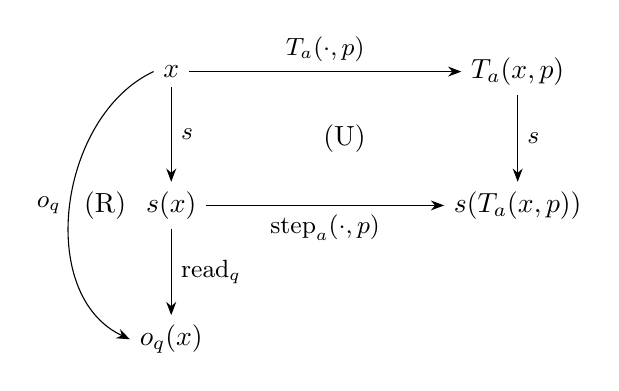
\begin{tikzpicture}[>=Stealth]
\node (x) at (0,0) {$x$};
\node (tx) at (4.4,0) {$T_a(x,p)$};
\node (sx) at (0,-1.7) {$s(x)$};
\node (stx) at (4.4,-1.7) {$s(T_a(x,p))$};
\node (q) at (0,-3.4) {$o_q(x)$};
\draw[->] (x) -- node[above] {\small $T_a(\cdot,p)$} (tx);
\draw[->] (x) -- node[right] {\small $s$} (sx);
\draw[->] (tx) -- node[right] {\small $s$} (stx);
\draw[->] (sx) -- node[below] {\small $\step_a(\cdot,p)$} (stx);
\draw[->] (sx) -- node[right] {\small $\rd_q$} (q);
\draw[->] (x.west) to[out=205,in=155] node[left] {\small $o_q$} (q.west);
\node at (2.2,-0.85) {(U)};
\node at (-0.84,-1.7) {(R)};
\end{tikzpicture}
\caption{The two identities of a summary statistic. Encoding after an action equals updating the
encoding (U), and reading the encoding answers the query that the curved arrow asks of the state
directly (R). A store that keeps $s(x)$ can follow the middle row, and read every answer from it,
without ever holding $x$.}\label{fig:square}
\end{figure}

\Cref{fig:square} draws (U) and (R). Condition (C) belongs to the machine rather than to the
statistic, but it is checked with it, because the other three conditions are claimed only on $X$. A
\emph{history} is a term built from states of $X$ by actions and merges. Write $\llbracket
h\rrbracket\in X$ for its value, the state it evaluates to, and $\llbracket h\rrbracket_S\in S$ for
the value obtained by replacing each state $x$ by $s(x)$, each action by its abstract update and
each merge by its abstract merge.

\begin{proposition}[Sufficiency]\label{prop:suff}
For a summary statistic and every history $h$, $s(\llbracket h\rrbracket)=\llbracket
h\rrbracket_S$. In particular $o_q(T_w x)=\rd_q(\step_w(s(x)))$ for every word $w$ and query $q$,
and two states with equal statistic values answer every query alike after every history.
\end{proposition}

\begin{proof}
By induction on $h$. For a state $x$ both sides are $s(x)$. For $h=a_p(h')$, the value
$\llbracket h'\rrbracket$ lies in $X$ by (C) and induction, so (U) and the induction hypothesis
give $s(T_a(\llbracket h'\rrbracket,p))=\step_a(s(\llbracket h'\rrbracket),p)=\step_a(\llbracket
h'\rrbracket_S,p)$. Merges are the same with (M). The second statement follows with (R).
\end{proof}

\plain If reading the summary answers each question and updating the summary keeps pace with every
operation, then the summary answers every question after any history, and the store needs nothing
else.

\begin{remark}[Relation to the specification]\label{rem:descent}
Condition (R) says that the current defect $\dnow$ of the encoding is zero, with decoder $\rd_q$,
and (U) that the update defect $\dupd$ is zero, with abstract update $\step_a$; Proposition~4.5 of
the specification says that such maps exist when the defects vanish and that together they make the
behavioral defect zero \cite[Section~4.2]{spec}. A summary statistic is that proposition with the
maps supplied. On an enumerated carrier the difference is small. On a symbolic carrier it changes
the shape of the obligations: the defect form compares pairs of states with equal codes and asks
whether some function exists, while the certificate form is one identity per action and per query
over a single state, a universally quantified formula that a decision procedure handles directly.
The supplied maps are also an implementation: the store keeps $s(x)$ and applies $\step_a$. The
cost-aware CoDD paper's \emph{implemented concept} packages an encoder, update procedures,
consumer queries, guards, laws, certificates and resource records \cite[Definition~6.1]{codd}; a
summary statistic is the part of such a package that a checker can establish exactly.
\end{remark}

\subsection{The coarsest statistic}

A \emph{context} is a history with one hole. Two states are \emph{behaviorally equivalent},
$x\approx y$, when every context $C$ and query $q$ give $o_q(\llbracket C[x]\rrbracket)=
o_q(\llbracket C[y]\rrbracket)$. Without merges, contexts are words, and this is the relation of
Part I's \code{MinimizeForQueries}.

\begin{proposition}[The coarsest statistic]\label{prop:coarsest}
\leavevmode
\begin{enumerate}[label=(\roman*)]
\item Every summary statistic refines $\approx$: $s(x)=s(y)$ implies $x\approx y$.
\item The quotient map $x\mapsto[x]_{\approx}$ is a summary statistic.
\item A summary statistic is coarsest, that is $s(x)=s(y)$ exactly when $x\approx y$, if and only
  if any two states with different values are separated by some context and query. The coarsest
  statistic is unique up to renaming its values.
\end{enumerate}
\end{proposition}

\begin{proof}
(i) is Proposition~\ref{prop:suff} applied inside contexts. For (ii), $x\approx y$ implies
$T_a(x,p)\approx T_a(y,p)$, $m(x,z)\approx m(y,z)$ and $m(z,x)\approx m(z,y)$, since a context of
the result is a context of the argument, and implies $o_q(x)=o_q(y)$ through the empty context; so
updates, merges and reads are well defined on classes. (iii) follows from (i) and (ii).
\end{proof}

On a finite machine the coarsest statistic is computed by partition refinement, which is the
content of Part I's \code{MinimizeForQueries} and of Theorem~4.2 of the goal-preservation paper
\cite{goalpres}. On an infinite carrier there is no general algorithm. The approach here is to
propose a statistic, check (C), (R), (U) and (M) with a solver, and establish minimality by giving
a separating context as a function of the two values, whose correctness is again a solver
obligation. In the engine statistic of Pattern~1, for example, two open items with ages $v<v'\le
7$ are separated by waiting $7-v'+(v'-v)/2$ days, after which the first is still within the
seven-day cap and the second is past it.

The coarsest statistic is the smallest exact memory, and it need not be the cheapest to maintain.
The cost-aware CoDD paper observes that among sufficient encodings one with more values, or with
redundancy, may have much cheaper operations, since the quotient does not order its
implementations by runtime or memory \cite[Section~6.2]{codd}. Its example also shows the update
language deciding what suffices: under insertions and deletions the bit ``some object remains''
cannot be updated exactly, and recomputing it means scanning the whole population, while an
incremental count, which keeps more distinctions, is updated in constant time.
Section~\ref{sec:dk} meets the same effect of deletions with sources of evidence.

\subsection{Checking a statistic}\label{sec:checking}

The proposed request \code{CheckStatistic} turns a \code{Statistic} declaration into obligations,
one \emph{closed} and one \emph{step} obligation for each action entry, one \emph{read} obligation
for each query, and one \emph{closed} and one \emph{merge} obligation for each merge entry. A
declaration that lacks a \code{Step} for some action, a \code{Read} for some query or a
\code{MergeStep} for some merge is rejected as invalid input. Each obligation has the form
``for every state and parameter in the declared carriers, $\varphi$''. \Cref{tab:methods} lists the
three ways it can be established and the statuses they give.

\begin{table}[ht]
\centering\small
\begin{tabularx}{\textwidth}{>{\raggedright\arraybackslash}p{3.0cm}>{\raggedright\arraybackslash}X>{\raggedright\arraybackslash}p{3.3cm}}
\toprule
Method & How & Status\\
\midrule
Symbolic & The negation of each obligation is given to a solver for the carriers' theories: linear
or nonlinear real arithmetic, Booleans and enumerated symbols, finite sets with cardinality over an
uninterpreted sort. Unsatisfiable for every obligation: the statistic holds for every state. A
model of some negation: a counterexample, replayed by evaluation. & Conditional on the solver
until a proof of unsatisfiability is checked, then Checked; Refuted with a replayed witness;
Unknown at the solver's limit (Section~\ref{sec:backends})\\
Through a finite model & A map into one of Part I's finite models that commutes with the actions,
possibly up to stuttering (Section~\ref{sec:c1}); the finite model is then checked exhaustively as
in
Part I. & Conditional on the solver that checked the map, then Checked once its proof is
checked; Refuted with a realized run; Unknown when an abstract
counterexample cannot be realized\\
Testing & The obligations are evaluated on sampled or logged states. A failure is a counterexample;
success bounds the rate of failing states under the sampling distribution
(Section~\ref{sec:zero}). & Refuted, or Estimated\\
\bottomrule
\end{tabularx}
\caption{Three ways to establish a statistic's obligations.}\label{tab:methods}
\end{table}

Testing never yields Checked. The cost-aware CoDD paper's acceptance gate puts the rule in one
sentence: ``A finite test suite should not be labeled a proof over untested states''
\cite[Appendix~C.3]{codd}. The symbolic method has one practical detail of its own. The solvers
decide the obligations over the real numbers. A verdict of unsatisfiability over the reals holds
over the rationals, which are what MeTTaDinC's \code{Rational} carriers contain, but a model must have
rational values before it can be replayed, and a model with irrational values gives Unknown.

In the bundle every item statistic of the modules was checked twice: by Z3 on encodings written by
hand in \fpath{models/smt_live.py} and \fpath{models/p3_live.py}, and by cvc5 on encodings that the
reference evaluator \fpath{ls_eval.py} builds from the module text. The keyed statistics follow by
lifting (Section~\ref{sec:c3}). The two encodings were written separately, so an error in
transcribing a module would show up as a disagreement. There were none. Agreement between two
solvers is evidence and not a proof, and neither solver's proof is checked here, so the statistics
are reported as Conditional, with the assumption that cvc5 answered correctly and Z3's agreement
recorded beside it (Section~\ref{sec:backends}).

\section{Five constructions}\label{sec:constructions}

The five constructions below cover every pattern of this part. Each comes with a proposition that
says when it is exact, and the last one says how to bound the error of statistics that are not.

\subsection{Abstraction to a finite model}\label{sec:c1}

The first construction reuses Part I. Many live states differ only in real values that the consumers
read through thresholds: a claim's confidence enters the goals only through whether it is at least
$4/5$, deadline pressure only through whether it is at least $1/2$. A map $h$ that sends each live
state to its classes lands in a finite model, and if the actions respect the classes, Part I's
exhaustive verdicts about the finite model carry over.

\begin{proposition}[Abstraction to a finite model]\label{prop:stutter}
Let $M$ be a machine with carrier $X$, $N$ a machine with carrier $Y$, and $h\colon X\to Y$ a map
such that every query $q$ of $M$ is a query of $N$ with $o_q=o'_q\circ h$, and every action family
$a$ of $M$ has a counterpart $\bar a$ in $N$.
\begin{enumerate}[label=(\roman*)]
\item (Lockstep.) Suppose $h(T_a(x,p))=T'_{\bar a}(h(x))$ for all $x$ and $p$, and that every
  merge entry $m$ of $M$ has a counterpart $m'$ in $N$ with $h(m(x,y))=m'(h(x),h(y))$. Then $h$, with
  $\step_a=T'_{\bar a}$, $\mstep_m=m'$ and $\rd_q=o'_q$, is a summary statistic of $M$. Hence
  $o_q(T_wx)=o'_q(T'_{\bar w}h(x))$ for every word $w$, where $\bar w$ replaces each action of $w$ by
  its counterpart, so every claim about $N$'s answers after words of counterpart actions from
  $h(x)$ holds for $M$ after the corresponding words from $x$. Claims about words of $N$ that
  contain other actions do not transfer.
\item (Stuttering.) If $h(T_a(x,p))\in\{h(x),\,T'_{\bar a}(h(x))\}$ for all $x$ and $p$, then for
  every run $x_0,x_1,\ldots,x_n$ of $M$ the sequence $h(x_0),\ldots,h(x_n)$ with consecutive
  repetitions removed is a run of $N$. Every state reachable from $x_0$ maps to a state reachable from
  $h(x_0)$, and each of the three safety forms of the specification's \code{Simulation} library that
  holds in $N$ from $h(x_0)$ holds in $M$ from $x_0$. The forms are \code{Shows} (no reachable state
  shows a given answer), \code{EnterFrom} (no transition enters a state showing one answer from a
  state showing neither it nor a second one) and \code{ReachWithin} (no run of at most $k$ steps
  reaches a state showing a given answer) \cite[Section~8.2]{spec}.
\end{enumerate}
\end{proposition}

\begin{proof}
(i) is Definition~\ref{def:stat} with the maps named, and the identity for words is
Proposition~\ref{prop:suff}. For (ii), each step of the run either leaves
the image fixed or moves it by a step of $N$; removing the fixed steps leaves a run of $N$, so
reachable states map to reachable states, and \code{Shows} transfers because related states answer
alike. A step of $M$ that leaves the image fixed changes no query answer, so it cannot be a
transition that \code{EnterFrom} forbids; any other step is matched by a step of $N$ with the same
answers at both ends. A run of $M$ is never shorter than its image, which gives
\code{ReachWithin}.
\end{proof}

Stuttering is the natural relation for real-valued state. A small increment of evidence leaves a
claim's class unchanged; a larger one moves it across the threshold, which is a step of the finite
model. The converse transfer, from a violation in $N$ to one in $M$, holds only when the abstract
run can be realized by concrete parameters. The checker tries to realize it one step at a time,
asking the solver for a parameter that moves the live state into the next abstract state; a realized
run is a Refuted witness about $M$, and an abstract run that cannot be realized gives Unknown. The
specification's counterexample-guided loop also returns Unknown for a spurious abstract run,
together with a predicate that refines the abstraction \cite[Section~8.2]{spec}; the checker of this
part stops at Unknown and leaves the refinement step open. Pattern~6 uses both directions.

\subsection{Saturation at thresholds}\label{sec:c2}

The second construction handles clocks. An item's age grows with every wait; queries compare it with
thresholds, such as the goal engine's seven-day cap or a two-day follow-up window. An age beyond the
largest threshold can never change an answer again, because ages only grow, so the statistic can
replace it by a marker.

\begin{proposition}[Saturation]\label{prop:sat}
Let a machine have a clock component $a\in\Q_{\ge 0}$ that every wait $d\ge 0$ advances to $a+d$,
that other actions leave unchanged, and that the queries read only through comparisons $a\le
\theta_i$ with thresholds $\theta_1<\cdots<\theta_k$, together with components the clock does not
affect. Write $\theta=\theta_k$.
\begin{enumerate}[label=(\roman*)]
\item The map $\sat_\theta(a)=(a>\theta,\ a\cdot[a\le\theta])$, with the abstract wait that sends
  $(t,v)$ to $(t\lor v+d>\theta,\ (v+d)\cdot[\lnot t\land v+d\le\theta])$, together with the other
  components unchanged, is a summary statistic.
\item If the query at $\theta$ is read on a set of live items that waits do not leave, then two live
  ages $v<v'\le\theta$ are separated by waiting $\theta-v'+(v'-v)/2$, and an age at most $\theta$ is
  separated from the marker immediately; on live items the statistic is the coarsest that keeps the
  other components.
\item Adding a query with a threshold $\theta'>\theta$ makes $\sat_\theta$ inadequate: a live
  age in $(\theta,\theta']$ and a live age above $\theta'$ share the value $(\mathit{true},0)$ and
  answer the new query differently. The coarsest statistic then saturates at $\theta'$.
\end{enumerate}
\end{proposition}

\begin{proof}
(i) If $a>\theta$ then $a+d>\theta$, and if $a\le\theta$ the new value is decided by $a+d$, so the
abstract wait commutes with encoding; each comparison $a\le\theta_i$ is read as
$\lnot t\land v\le\theta_i$. (ii) After the wait the first age is $\theta-(v'-v)/2\le\theta$ and the
second $\theta+(v'-v)/2>\theta$. (iii) is immediate.
\end{proof}

\plain Remember an age only until the last deadline any goal can still read; once a goal with a
later deadline is added, the memory must keep ages that long.

The rule in (iii) is the live form of a transport rule of the specification: adding a query resumes
refinement from the current memory and can only make it finer, and removing one lets it coarsen
\cite[Section~4.8]{spec}. When a flag makes every clock value equivalent, as a closed item is
neither suggested nor open whatever its age, the coarsest statistic also forgets the clock for those
items; the statistics of Patterns~1 and~5 do this by resetting the value of a closed item to a
fixed one. If, moreover, a flagged item and an item past the last threshold answer every query
alike from then on, the coarsest statistic merges them too. The engine statistic of Pattern~1 does;
the statistic of Pattern~5 keeps them apart because it keeps the open flag.

\subsection{Keys, counts and histograms}\label{sec:c3}

The third construction lifts an item statistic to a store. A store holds finitely many items under
identifiers. Some actions address one item, such as a reply to item $k$; some apply to every item,
such as the passage of time; insertions add items. Queries ask about one item or count items.

\begin{proposition}[Lifting]\label{prop:lift}
Let $(S,s,\step,\rd)$ be a summary statistic of the item machine. On the store machine, the keyed
statistic $s^K(\sigma)=(k\mapsto s(\sigma(k)))$ is a summary statistic for the item queries
$(q\ k)$ and the counts $\#\{k:o_q(\sigma(k))\}$ of Boolean queries: insertion of $x$ under $k$ sets
$k\mapsto s(x)$, an item action at $k$ applies $\step_a$ at $k$, a global action applies $\step_a$
at every key, $(q\ k)$ reads $\rd_q(s^K(\sigma)(k))$, and a count counts the keys whose value reads
true. Suppose moreover that $S$ is finite, that insertions use fresh keys, that global actions
apply the same $\step_a$ everywhere, and that item actions address an item by its statistic value
rather than by its key, acting on some key with that value. Then the histogram
$n_c=\#\{k:s(\sigma(k))=c\}$ is a summary statistic for the counts, whichever such key an item
action acts on.
\end{proposition}

\begin{proof}
Every identity holds key by key. For the histogram, inserting $x$ under a fresh key adds one to
$n_{s(x)}$, a global action sends $n$ to $n'_{c'}=\sum_{c:\step_a(c)=c'}n_c$, an item action at
value $c$ moves one unit from $c$ to $\step_a(c)$ whichever key with value $c$ it acts on, and a
count is $\sum_{c:\rd_q(c)}n_c$.
\end{proof}

The proposition has a premise that an implementation must check rather than assume: the item
statistic is a statistic of the store's item machine, the machine whose states the store holds and
whose queries its consumers ask. A statistic of another machine over the same states and actions
answers only that machine's queries. Pattern~1 has an example. The engine's coarsest statistic is a
statistic of \code{EngineTime}, which asks only whether to suggest an item, and it gives the items
$(8,\mathrm{false},0)$ and $(8,\mathrm{true},0)$ the same code, although the first is open and the
second closed. Lifted as an index of the store of \code{ItemTime} items, whose consumers also ask
whether an item is open, it would certify an index that cannot answer that question. The proposed
\code{Keyed} declaration therefore states which machine its index serves. Without further fields
the item statistic must be a statistic of the store's item machine, and anything else is
InvalidInput; to index a view of the items, such as \code{EngineTime}, the declaration names it with
\code{(View EngineTime)}, the view must have the store's states and declare its actions as those of
the store's item machine, and the lifted result is bound to the view's queries alone. A consumer of
the other queries then finds no certificate for them. The bundle carries both declarations, and the
first is one of its negative fixtures (Section~\ref{sec:lp1}).

A histogram over a real clock is not finite, but buckets give bounds. If the open items of each
addressee are counted by creation day, the number that are open and at most seven days old at time
$t$ is at least the count of the days that lie entirely within the last seven days and at most that
count plus the count of the day on which the window begins. Pattern~1 measures the width of these
bounds on a simulated workload.

\subsection{Identity-bounded sets}\label{sec:dk}

The fourth construction counts distinct identifiers from an open set. Part I's evidence consumers
ask whether any contradicting source has reported, how many distinct supporting sources there are
up to two, and whether at least two distinct contradicting sources have reported. On three sources
the coarsest memory was, for each polarity, ``no source, the only source so far, or two or more''.
With an unbounded set of sources the same memory is the identity-bounded set.

\begin{definition}[$D_K$]
For a positive integer $K$ and a finite set $A$ of identifiers, $D_K(A)=A$ if $|A|<K$ and
$D_K(A)=\Many$ otherwise. On values, insertion, union and size are
\begin{align*}
\mathrm{CapInsert}_K(x,A)&=D_K(A\cup\{x\}), & \mathrm{CapInsert}_K(x,\Many)&=\Many,\\
\mathrm{CapUnion}_K(A,B)&=D_K(A\cup B), & \mathrm{CapUnion}_K(c,d)&=\Many\ \text{if $c$ or $d$ is
$\Many$},\\
\mathrm{CapSize}_K(A)&=|A|, & \mathrm{CapSize}_K(\Many)&=K.
\end{align*}
\end{definition}

\begin{proposition}[Identity-bounded sets]\label{prop:dk}
\leavevmode
\begin{enumerate}[label=(\roman*)]
\item The identities
  \begin{gather*}
  D_K(A\cup\{x\})=\mathrm{CapInsert}_K(x,D_K(A)),\quad
  D_K(A\cup B)=\mathrm{CapUnion}_K(D_K(A),D_K(B)),\\
  \min(K,|A|)=\mathrm{CapSize}_K(D_K(A))
  \end{gather*}
  hold, so $D_K$ is a summary statistic, with merges, for every query that reads $\min(K,|A|)$,
  including thresholds $|A|\ge j$ for $j\le K$.
\item Under insertions it is the coarsest such statistic: two different values are separated by
  inserting at most one identifier.
\item $\mathrm{CapUnion}_K$ is commutative, associative and idempotent, so replicas that exchange
  values in any order and any number of times converge to the value of the union of all they have
  seen.
\item Under withdrawals of sources $D_K$ is not a statistic: for $K=2$, the sets $\{a,b\}$ and
  $\{a,b,c\}$ share the value $\Many$, and after $a$ and $b$ are withdrawn one is empty and the other
  is not.
\end{enumerate}
\end{proposition}

\begin{proof}
(i) If $|A|\ge K$ then $|A\cup\{x\}|\ge K$; otherwise both sides are $D_K(A\cup\{x\})$. Union is the
same, and the read is immediate. (ii) Values of different size are separated at once. Two different
sets $A\ne B$ of the same size $j<K$ have an element $x\in A\setminus B$ (or the reverse); inserting
$x$ gives sizes $j$ and $j+1\le K$. A set of size below $K$ and $\Many$ are separated at once.
(iii) The values are the sets of size below $K$ together with a top element, and
$\mathrm{CapUnion}_K$ is the join of this semilattice. (iv) is the example.
\end{proof}

Part (iii) makes $D_K$ a state-based conflict-free replicated data type \cite{crdt}: two forks of
an evidence store that share part of their history merge exactly, however much they share. Totals
of incidents do not have this property, since adding the totals of two forks counts the shared
history twice; Pattern~3 measures how often. Part (iv) is the cost-aware CoDD paper's observation
about deletions in another setting \cite[Section~6.2]{codd}: a store from which sources can be
withdrawn must keep the full set of distinct sources, or per-source counts if single incidents can
be withdrawn.

\subsection{Approximate and one-sided statistics}\label{sec:c5}

The fifth construction is for statistics that are not exact, either because the implementation
rounds or because an exact statistic would be too large. Two kinds of claims remain available: a
bound on the error, and a guarantee that the error has one sign.

\begin{proposition}[Error propagation]\label{prop:error}
Let the statistic values carry a metric $d$, let each abstract update be $L$-Lipschitz, that is
$d(\step(u),\step(v))\le L\,d(u,v)$ for all values $u,v$, and let an
implementation start within $\varepsilon_0$ of the exact value and add an error of at most
$\varepsilon$ per update, $d(\hat s_{t+1},\step(\hat s_t))\le\varepsilon$. Then after $t$ updates
\[
d(\hat s_t,s_t)\le L^t\varepsilon_0+\varepsilon(1+L+\cdots+L^{t-1}).
\]
For $L<1$ the error stays below $\varepsilon_0+\varepsilon/(1-L)$ forever. For $L=1$ it can grow by
$\varepsilon$ per update, and recomputing the value exactly from the records every $R$ updates keeps
it below $R\varepsilon$ plus the error of the recomputed value.
\end{proposition}

\begin{proof}
$d(\hat s_{t+1},s_{t+1})\le d(\hat s_{t+1},\step(\hat s_t))+d(\step(\hat s_t),\step(s_t))\le
\varepsilon+L\,d(\hat s_t,s_t)$; unroll the recursion.
\end{proof}

This is the affine contract of the specification's implementation checks, $d\le L\,d_{\mathrm{in}}+
\eta$, composed along a run by the composition rule for grades \cite[Proposition~9.1]{spec}: $t$
updates with grade $(L,\varepsilon)$ compose to grade $(L^t,\varepsilon(1+\cdots+L^{t-1}))$. For a
crisp consumer that reads a threshold, an error bound $\delta$ on the statistic makes the answer
exact whenever the stored value is farther than $\delta$ from the threshold; within $\delta$ of the
threshold the right report is Unknown, with the component's declared fallback.
Two simulations in the bundle show both regimes. Attention that decays by a factor $1/2$ per tick
and is rounded to an integer after every update has $L=1/2$ and $\varepsilon=1/2$, so its error is
at most $1$; over $5{,}000$ updates with random boosts the largest error was $0.90$. A running total
of usage weights has $L=1$. The weights are in hundredths and each is rounded half up to a whole
unit, which adds an error of $1/200$ per update on average; after $100{,}000$ updates the plain
total was off by $512.09$, with a largest error of $534.8$ along the way, while recomputing it from
the records every $100$ updates kept the error below its bound of $50.5$, at $12.44$.

\begin{proposition}[One-sided statistics]\label{prop:onesided}
Let a summary $\hat s$ come with a read $\hat r_q$ that answers \emph{no} or \emph{maybe} for a
Boolean query $q$, and suppose $\hat r_q(\hat s(x))=$ \emph{maybe} whenever $q(x)$ holds. Let a
consumer take its safe action, such as revalidating, keeping or withholding, whenever the answer is
\emph{maybe}, and its other action when the answer is \emph{no}. Then the consumer satisfies every
guarantee of the form ``whenever $q$ holds, the safe action is taken''. More generally, it
satisfies every property that holds for the consumer that reads $q$ exactly and that is preserved
when the safe action is taken in additional states. The cost is the safe action taken in the states
where $q(x)$ is false and the answer is \emph{maybe}.
\end{proposition}

\begin{proof}
If $q(x)$ holds, the answer is \emph{maybe}, so the safe action is taken. The consumer reading
$\hat r_q$ differs from the exact consumer only on states where $q(x)$ is false and the answer is
\emph{maybe}, and there it takes the safe action in place of the other one.
\end{proof}

A Bloom filter is one-sided for membership: an inserted element sets its $k$ bits, and bits are
never cleared, so a member always reads \emph{maybe}. That part is an exact property of the data
structure, of the kind a symbolic check establishes. Its rate of false positives, about $(1-e^{-kn/m})^k$ for $n$ elements in $m$ bits with
ideal hash functions \cite{bloom}, depends on the hash functions and is an Estimated property.
A Count--Min sketch with nonnegative updates is one-sided in the same way, since it never
underestimates a frequency, but its bound on the overestimate holds only with a stated probability
over its hash functions \cite{countmin}. HyperLogLog's estimate of a number of distinct elements
can err in either direction, again within a bound that holds with a stated probability \cite{hll}.
Those probabilistic bounds are Estimated claims and suit only empirical consumers.
\section{Claims about the running system}\label{sec:estimates}

A summary statistic is sufficient relative to its input events. If the detector that decides
whether a message is a reply misses one, the open-item statistic faithfully keeps a settled item
open; if the parser drops the source of a judgment, the evidence statistic never sees it. What the
language model does with a context block is outside every declaration as well. These are quantities
of the running system, and they are rates. The goal-preservation paper draws the line in the same
place: ``Exact program proofs and statistical response audits solve different parts of the problem.
A program proof can establish which states and transitions are possible; sampling can estimate
response probabilities in those states'' \cite[Section~6]{goalpres}.

\subsection{What an Estimated claim states}

The specification asks an Estimated result to name its estimand, its estimator, the sampling
protocol, the sample size, an error bound with its failure probability, and the rule by which
several estimates are combined \cite[Section~7.4]{spec}. It also names the population the receipts
sample, the rule that selects which units become rows and when, and the version of the policy under
which the rows were produced, because a rate measured under one policy says nothing about another
until an argument carries it over. The streams of this part's modules declare these three fields,
and \code{EstimateRate} reports them with its interval. For the claims of this part the raw material
is a \emph{receipt}: a record, written when a context block is built or a suggestion is made, of
which consumers were served. Part I proposed the receipt formats \cite[Appendix~C]{part1}. A column
of receipts is a sequence of binary events $X_1,X_2,\ldots$, such as ``the anchor consumer was missed
in snapshot $i$'', read in an order fixed before their labels are known. Write $\mu_i$ for the
conditional probability that $X_i=1$ given the events before it.

Two working assumptions appear below, and each result states which one it uses. The stronger is
that every $\mu_i$ equals one rate $p$, the probability of the event per snapshot under the current
workload; it is needed when an interval is read as an estimate of $p$. The weaker assumes nothing
about the $\mu_i$. A claim that the rate is below, or above, a fixed target is then a claim about
their running average, and Proposition~\ref{prop:onesided-cs} shows that the procedure below
supports it with the same guarantee.

\subsection{Rates from receipts}\label{sec:cs}

After $n$ events of which $S_n$ are failures, let
\[
M_n(p)=\frac{B(S_n+1,\ n-S_n+1)}{p^{S_n}(1-p)^{n-S_n}},
\]
where $B$ is the beta function. The numerator is the probability of the observed sequence averaged
over rates drawn uniformly from $[0,1]$, the denominator its probability under the rate $p$, so
$M_n(p)$ is a mixture of likelihood ratios. Under the rate $p$ it is a nonnegative martingale that
starts at $1$, and Ville's inequality gives $P(\exists n: M_n(p)\ge 1/\alpha)\le\alpha$. The set
\[
\mathrm{CS}_n=\{p: M_n(p)<1/\alpha\}
\]
is therefore a confidence sequence: with probability at least $1-\alpha$ it contains the true rate
at every $n$ at once \cite{robbins,howard}. Because $-S_n\log p-(n-S_n)\log(1-p)$ is convex in $p$,
each $\mathrm{CS}_n$ is an interval, and its ends are found by bisection. The proposed request
\code{EstimateRate} reports the interval at the last row of a frozen stream, with the stream's
digest. A simulation in the bundle checks the coverage: at level $0.05$, over $2{,}000$ runs of
$2{,}000$ events each, the true rate left the sequence at some point in $2.3$, $1.85$, $3.35$ and
$3.55$ percent of the runs for rates $0.01$, $0.05$, $0.2$ and $0.5$.

Claims at a promotion gate are usually one-sided: the rate of stale suggestions is below one in
twenty, or one policy misses a consumer more often than another. For such claims the rows need not
share a rate, and they need not be independent.

\begin{proposition}[One-sided claims without a common rate]\label{prop:onesided-cs}
Let $X_1,X_2,\ldots$ be binary events, $\mu_i$ the conditional probability that $X_i=1$ given
$X_1,\ldots,X_{i-1}$, and $\bar\mu_n=(\mu_1+\cdots+\mu_n)/n$. Fix a target $p^*\in(0,1)$ and let
$u_n$ and $\ell_n$ be the upper and lower ends of $\mathrm{CS}_n$ at level $\alpha$. Then
\begin{align*}
P\bigl(\exists n:\ u_n<p^*\ \text{and}\ \bar\mu_n\ge p^*\bigr)&\le\frac{p^*}{1/\alpha-1+p^*}\le\alpha,\\
P\bigl(\exists n:\ \ell_n>p^*\ \text{and}\ \bar\mu_n\le p^*\bigr)&\le\frac{1-p^*}{1/\alpha-p^*}\le\alpha.
\end{align*}
\end{proposition}

\begin{proof}
Write $S_n=X_1+\cdots+X_n$ and $L_n(\theta)=(\theta/p^*)^{S_n}((1-\theta)/(1-p^*))^{n-S_n}$, so that
$M_n(p^*)=\int_0^1L_n(\theta)\,d\theta$. The interval $\mathrm{CS}_n$ contains $S_n/n$, because
$M_n(S_n/n)\le 1<1/\alpha$: the likelihood ratio of any rate against the maximum-likelihood rate is
at most one. So $u_n<p^*$ implies $S_n/n<p^*$ and $M_n(p^*)\ge1/\alpha$. As a function of $\theta$,
$\log L_n$ is concave with its maximum at $S_n/n$, so for $\theta\ge p^*>S_n/n$ it is decreasing and
$L_n(\theta)\le L_n(p^*)=1$; hence $\int_{p^*}^1L_n\le 1-p^*$, and on the event in question
$A_n=\int_0^{p^*}L_n(\theta)\,d\theta\ge 1/\alpha-1+p^*$.

For $\theta<p^*$ put $\lambda=\log\bigl(\theta(1-p^*)/((1-\theta)p^*)\bigr)<0$. A short calculation gives
$L_n(\theta)=\exp\bigl(\lambda S_n-n\log(1-p^*+p^*e^\lambda)\bigr)$. Let
$Z_n(\lambda)=\exp\bigl(\lambda S_n-\sum_{i\le n}\log(1-\mu_i+\mu_ie^\lambda)\bigr)$. Since
$E[e^{\lambda X_i}\mid X_1,\ldots,X_{i-1}]=1-\mu_i+\mu_ie^\lambda$, $Z_n(\lambda)$ is a nonnegative
martingale with $Z_0=1$. The function $\mu\mapsto\log(1-\mu+\mu e^\lambda)$ is concave, and it is
decreasing because $\lambda<0$. Whenever $\bar\mu_n\ge p^*$, therefore,
$\sum_{i\le n}\log(1-\mu_i+\mu_ie^\lambda)\le n\log(1-\bar\mu_n+\bar\mu_ne^\lambda)\le
n\log(1-p^*+p^*e^\lambda)$, and so $L_n(\theta)\le Z_n(\lambda)$. Integrating over $\theta<p^*$,
$A_n\le\bar A_n=\int_0^{p^*}Z_n(\lambda(\theta))\,d\theta$, a nonnegative martingale that starts at
$p^*$. Ville's inequality gives $P(\exists n:\bar A_n\ge c)\le p^*/c$, and $c=1/\alpha-1+p^*$ gives
the first bound. The second follows by exchanging the labels $0$ and $1$, which turns $p^*$ into
$1-p^*$ and the lower end into an upper end.
\end{proof}

\plain A claim that a rate lies below a target keeps its guarantee when the receipts do not share
one rate, and even when they depend on each other. It is then a claim about the average, over the
receipts, of each receipt's probability of failing given the ones before it. At level $0.01$ and the
target $1/20$, the chance of a wrong claim of this kind is at most about $0.0005$. An interval read as
an estimate of a single rate still needs that rate to exist.

When the rate drifts, two-sided estimates need confidence sequences for the running average of the
conditional rates, which Howard and coauthors construct in a different form \cite{howard}. The unit
of a receipt still decides what a one-sided claim is about, since it decides what the average is an
average of. If one stale item is suggested on many consecutive days, an average over suggestions counts that
item once a day, and a claim about items needs one receipt per item. A simulation in the bundle
checks the proposition at level $0.05$: over $2{,}000$ runs of $2{,}000$ rows whose conditional
rates are all at least $1/20$, either shared, spread over $[1/20,3/20]$ or arranged so that a failure
is followed by another with probability $0.9$, the upper end fell below $1/20$ in at most $0.15$
percent of the runs, within the bound of $0.26$ percent.

\subsection{Zero failures and conformance replay}\label{sec:zero}

When no failure has been seen, $M_n(p)=1/((n+1)(1-p)^n)$, and the upper end of the sequence has a
closed form:
\[
U_n=1-\left(\frac{\alpha}{n+1}\right)^{1/n}\approx\frac{\ln(1/\alpha)+\ln(n+1)}{n}.
\]
The fixed-sample bound of Clopper and Pearson after $n$ events without a failure is
$1-\alpha^{1/n}\approx\ln(1/\alpha)/n$ \cite{clopper}, valid only if $n$ was fixed in advance.
\Cref{tab:zero} compares the two at $\alpha=0.01$. The anytime bound is two to four times larger,
and in exchange it may be read after every event.

\begin{table}[ht]
\centering\small
\begin{tabular}{rcc}
\toprule
Events without a failure & Anytime bound $U_n$ & Fixed-sample bound\\
\midrule
$100$ & $0.0881$ & $0.0450$\\
$1{,}000$ & $0.0114$ & $0.0046$\\
$10{,}000$ & $0.00138$ & $0.00046$\\
$100{,}000$ & $0.000161$ & $0.000046$\\
\bottomrule
\end{tabular}
\caption{Upper bounds on a failure rate at level $0.01$ after a run without failures.}\label{tab:zero}
\end{table}

The same bound serves \emph{conformance replay}. Part I tied each finite model to its code by
replaying recorded events through both \cite[Section~3.4]{part1}. For a live statistic the
corresponding check samples logged states at random, recomputes the statistic from the full records
and compares it with the stored value. A mismatch is a concrete bug, reported with the record. No
mismatch in $n$ samples bounds the mismatch rate by $U_n$. Testing the obligations of a statistic on
logged states, the third method of \cref{tab:methods}, gives an Estimated claim of exactly this
kind.

\subsection{Comparing two policies on the same snapshots}\label{sec:paired}

Two selection policies can be run on the same snapshots, one live and one in shadow, so their
receipts come in pairs. Snapshots on which both policies serve a consumer, or both miss it, say
nothing about which is better. On the \emph{discordant} snapshots, where exactly one misses, let
$b$ count those where the first misses and $c$ those where the second does. If the first policy
misses with probability $p_1$ and the second with $p_2$ per snapshot, then among discordant
snapshots the first misses with probability $r$, and $p_1-p_2$ has the sign of $r-1/2$. The
confidence sequence of \cref{sec:cs}, applied to the $b+c$ discordant snapshots, gives an interval
for $r$; an interval above one half says the first policy misses more often. This is the sequential
form of McNemar's test \cite{mcnemar}, and the proposed request \code{CompareRates} computes it. Read
as a one-sided claim against one half, it needs no common rate either: Proposition~\ref{prop:onesided-cs}
applies to the discordant snapshots in the order they occur.

\subsection{Monitors with fixed and mixed alternatives}\label{sec:monitors}

Part I's Pattern~8 watched the goal engine's stale suggestions with a monitor that multiplies, for
each suggestion, the likelihood ratio of a failing rate $q=1/5$ against the accepted rate
$p_0=1/20$ \cite[Section~11]{part1}. After $S$ stale suggestions among $n$ the monitor's current
value, its \emph{e-value}, is
\[
E_n=\left(\frac{q}{p_0}\right)^{S}\left(\frac{1-q}{1-p_0}\right)^{n-S}.
\]
For $q>p_0$ this is a nonnegative supermartingale whenever the true rate is at most $p_0$, so an
alarm at $1/\alpha$ has false-alarm probability at most $\alpha$. The monitor's power depends on the
true rate $p$ through the drift of $\log E_n$ per observation,
$p\ln(q/p_0)+(1-p)\ln((1-q)/(1-p_0))$. At $p=1/5$ the drift is $0.140$; at $p=3/10$ it is $0.296$;
at $p=1/10$, a rate twice the accepted one, it is $-0.016$. A monitor tuned for $1/5$ facing a rate
of $1/10$ accumulates evidence \emph{against} its alternative, and its e-value tends to zero.

The remedy is to average e-values over alternatives. A finite mixture averages the products for
several rates; the uniform mixture integrates over $q\in(p_0,1]$,
\begin{align*}
E_n&=\frac{1}{1-p_0}\int_{p_0}^{1}\left(\frac{q}{p_0}\right)^{S}
     \left(\frac{1-q}{1-p_0}\right)^{n-S}dq\\
   &=\frac{B(S+1,n-S+1)\,P(\mathrm{Beta}(S+1,n-S+1)>p_0)}{(1-p_0)\,p_0^{S}(1-p_0)^{n-S}}.
\end{align*}
An average of nonnegative supermartingales is again a nonnegative supermartingale, so the mixtures
keep the false-alarm guarantee. \Cref{tab:monitors} compares three monitors at level $0.01$ in
$1{,}000$ simulated runs of $2{,}000$ suggestions each: the fixed alternative $1/5$, the finite
mixture over $1/10$, $1/5$ and $2/5$, and the uniform mixture. Over $2{,}000$ runs at the accepted
rate $1/20$ the three raised false alarms in $0.45$, $0.50$ and $0.55$ percent of runs.

\begin{table}[ht]
\centering\small
\begin{tabular}{lccc}
\toprule
 & Fixed $q=1/5$ & Finite mixture & Uniform mixture\\
\midrule
Detected within $2{,}000$ at rate $1/10$ & $49.6\%$ & $100\%$ & $100\%$\\
Median detection time at rate $1/10$ & --- & $224$ & $310$\\
Median detection time at rate $1/5$ & $32$ & $37$ & $40$\\
False alarms at rate $1/20$ & $0.45\%$ & $0.50\%$ & $0.55\%$\\
\bottomrule
\end{tabular}
\caption{Three stale-suggestion monitors at level $0.01$.}\label{tab:monitors}
\end{table}

At the rate $1/5$ that the fixed monitor was built for, mixing delays the median detection by five
to eight suggestions; at the rate $1/10$ the fixed monitor detects in only half of the runs, and
both mixtures in all of them. The frozen stream \code{TenPercent}, $2{,}000$ suggestions at rate
$1/10$, shows how misleading a single run can be. The fixed monitor fires at suggestion $27$ after
an early streak of stale suggestions, which is a correct and valid alarm, but its e-value peaks at
$154.7$ and has fallen to about $1.2\times 10^{-14}$ by the end of the stream. The finite mixture
fires at suggestion $132$ and the uniform mixture at $152$, and both keep growing.

\subsection{Budgets and sample sizes}\label{sec:budgets}

Several Estimated claims made at once share their failure probability by a union bound unless a
joint procedure is declared \cite[Section~7.4]{spec}. Under GOLEM-Iter, Estimated results spend
from the gate's lifetime confidence budget and are committed by digest before the gate draws its
evaluation randomness, while certificates spend nothing, whether they are Checked or Conditional on
a solver \cite[Section~12.3]{part1}. Planning a
claim means knowing how many receipts it needs. \Cref{tab:sizes} gives the number of events from
which on the upper end of the confidence sequence at level $0.01$ stays below a target, when the
observed number of failures is the true rate times the number of events, rounded half up. The
rounding makes the upper end rise slightly each time the count steps up, so it first dips below the
target somewhat earlier, at $3{,}135$, $486$, $1{,}729$ and $1{,}147$ events. These are plug-in
sizes: the observed count varies around its mean, so at these sizes a claim is established only part
of the time, and a plan should fix the probability of success it wants and use the size that
achieves it, which is larger.

\begin{table}[ht]
\centering\small
\begin{tabular}{ccr}
\toprule
True rate & Target for the upper end & Events needed\\
\midrule
$0.01$ & $0.02$ & $3{,}275$\\
$0.05$ & $0.10$ & $514$\\
$0.05$ & $0.075$ & $1{,}811$\\
$0.20$ & $0.25$ & $1{,}179$\\
\bottomrule
\end{tabular}
\caption{Receipts needed before the upper bound stays below a target, at level
$0.01$.}\label{tab:sizes}
\end{table}

\plain A rate can be watched continuously and reported at any moment if it is estimated with a
confidence sequence; a run without failures bounds the rate by about $(4.6+\ln n)/n$ at level
$0.01$; two policies are best compared on the same snapshots; and a monitor should average over the
failure rates it might face rather than assume a single one.
\section{The patterns on live memory}\label{sec:patterns}

Each pattern of Part I is worked again below. Every module of this section except the receipts
module of Pattern~8 declares its carriers symbolically, with \code{(Carriers Symbolic)} in its
profile, and every symbolic request is answered for all states of those carriers; the receipts
module is stochastic and reads frozen streams. The results quoted are those of the bundle's oracle,
which obtains each symbolic verdict from both solvers and replays every witness. A verdict that rests
on a solver's answer of unsatisfiability is reported as Conditional on cvc5, the solver the reference
evaluator calls, because no proof of it is checked (Section~\ref{sec:backends}); Z3 agrees with every
such verdict on its own encodings. Refutations are Refuted, since their witnesses are replayed by
evaluation, and verdicts computed in exact arithmetic without a solver are Checked. A request that
applies a certificate to the wrong object is InvalidInput; the modules carry two such requests as
negative fixtures, and the oracle adds a third, a copy of a stream changed under its declared
digest, which the evaluator refuses (Section~\ref{sec:lp8}).

\subsection{Pattern 1: open items in real time}\label{sec:lp1}

\paragraph{The problem.} Part I modeled an open item by its age in whole days, from zero to seven
with one more value for anything older, and the time since its closing reply in four coarse
steps. That was enough to show that closing
items by what a recall window shows reopens them as replies age out of the window. The live engine
works in real time: an item is created at some moment, a reply may be detected at any later moment,
the engine asks at arbitrary times whether an item is open and at most seven days old, and the
commitment record asks whether it is open. The question is which record design answers both, for
every timing and for a store of any size.

\paragraph{The module.} An item is a triple of its age, whether it is closed, and the time since
the closing reply, with the second time at most the first. Waiting is a family of actions over all
nonnegative durations. The module declares three statistics and the window view, and lifts two of
the statistics to a keyed store.

\begin{lstlisting}[style=mettamod]
(DC.Module LiveOpenItems
  (Profile (Dynamics Deterministic) (Values Crisp) (Carriers Symbolic))
  (Use RationalArith Families Statistics)              ; PROPOSED libraries
  (Carrier Rat  (Of Rational) (All))
  (Carrier Flag (Of Bool) (Enum False True))
  (Map nonnegative (From Rational) (To Bool) (Body ($x) (Le 0 $x)))
  (Carrier Days (Of Rational) (Subset Rat nonnegative))
  ;; an item: (age in days, closed, days since the closing reply)
  (Carrier Raw  (Of (Tuple Rational Bool Rational)) (Product Days Flag Days))
  (Map well-formed (From (Tuple Rational Bool Rational)) (To Bool)
    (Cases ((Tuple $a $c $e) (Le $e $a))))
  (Carrier Item (Of (Tuple Rational Bool Rational)) (Subset Raw well-formed))

  ;; how an item changes, and what its users ask
  (Map wait (Parameters ($d Days)) (From Item) (To Item)
    (Cases ((Tuple $a $c $e) (Tuple (Add $a $d) $c (Add $e $d)))))
  (Map on-reply (From Item) (To Item)
    (Cases ((Tuple $a $c $e) (Tuple $a True (If $c $e 0)))))
  (Map suggest (From Item) (To Bool) (Cases ((Tuple $a $c $e) (And (Not $c) (Le $a 7)))))
  (Map open    (From Item) (To Bool) (Cases ((Tuple $a $c $e) (Not $c))))
  (Machine ItemTime (States Item) (Observe suggest suggest) (Observe open open)
    (Action (wait $d) (wait $d) (For $d Days))       ; PROPOSED For over Days
    (Action reply on-reply))
  (Machine EngineTime (States Item) (Observe suggest suggest) (ActionsOf ItemTime))

  ;; the event statistic: the age and whether the item is closed
  (Map event-stat (From Item) (To (Tuple Rational Bool))
    (Cases ((Tuple $a $c $e) (Tuple $a $c))))
  (Map event-wait (Parameters ($d Days)) (From (Tuple Rational Bool))
    (To (Tuple Rational Bool)) (Cases ((Tuple $a $c) (Tuple (Add $a $d) $c))))
  (Map event-reply (From (Tuple Rational Bool)) (To (Tuple Rational Bool))
    (Cases ((Tuple $a $c) (Tuple $a True))))
  (Map event-suggest (From (Tuple Rational Bool)) (To Bool)
    (Cases ((Tuple $a $c) (And (Not $c) (Le $a 7)))))
  (Map event-open (From (Tuple Rational Bool)) (To Bool) (Cases ((Tuple $a $c) (Not $c))))
  (Statistic EventStat (Of ItemTime) (Encode event-stat)          ; PROPOSED Statistic
    (Step (wait $d) (event-wait $d) (For $d Days)) (Step reply event-reply)
    (Read suggest event-suggest) (Read open event-open))

  ;; the coarsest statistic for both users: closed, or the age of an open item saturated
  ;; at seven days (the flag is true once the age is past seven days)
  (Map joint-stat (From Item) (To (Tuple Bool Bool Rational))
    (Cases ((Tuple $a $c $e)
      (Tuple $c (And (Not $c) (Lt 7 $a)) (If (And (Not $c) (Le $a 7)) $a 0)))))
  (Map joint-wait (Parameters ($d Days)) (From (Tuple Bool Bool Rational))
    (To (Tuple Bool Bool Rational))
    (Cases ((Tuple $c $t $v)
      (Tuple $c (And (Not $c) (Or $t (Lt 7 (Add $v $d))))
             (If (And (Not $c) (Not (Or $t (Lt 7 (Add $v $d))))) (Add $v $d) 0)))))
  (Map joint-reply (From (Tuple Bool Bool Rational)) (To (Tuple Bool Bool Rational))
    (Cases ((Tuple $c $t $v) (Tuple True False 0))))
  (Map joint-suggest (From (Tuple Bool Bool Rational)) (To Bool)
    (Cases ((Tuple $c $t $v) (And (Not $c) (Not $t)))))
  (Map joint-open (From (Tuple Bool Bool Rational)) (To Bool)
    (Cases ((Tuple $c $t $v) (Not $c))))
  (Statistic JointStat (Of ItemTime) (Encode joint-stat)
    (Step (wait $d) (joint-wait $d) (For $d Days)) (Step reply joint-reply)
    (Read suggest joint-suggest) (Read open joint-open))

  ;; the coarsest statistic for the engine alone: dead (closed or past seven days), or
  ;; the age of a live item
  (Map engine-stat (From Item) (To (Tuple Bool Rational))
    (Cases ((Tuple $a $c $e) (Tuple (Or $c (Lt 7 $a)) (If (Or $c (Lt 7 $a)) 0 $a)))))
  (Map engine-wait (Parameters ($d Days)) (From (Tuple Bool Rational))
    (To (Tuple Bool Rational))
    (Cases ((Tuple $x $v)
      (Tuple (Or $x (Lt 7 (Add $v $d))) (If (Or $x (Lt 7 (Add $v $d))) 0 (Add $v $d))))))
  (Map engine-reply (From (Tuple Bool Rational)) (To (Tuple Bool Rational))
    (Cases ((Tuple $x $v) (Tuple True 0))))
  (Map engine-suggest (From (Tuple Bool Rational)) (To Bool)
    (Cases ((Tuple $x $v) (Not $x))))
  (Statistic EngineStat (Of EngineTime) (Encode engine-stat)
    (Step (wait $d) (engine-wait $d) (For $d Days)) (Step reply engine-reply)
    (Read suggest engine-suggest))

  ;; what a two-day recall window shows: the age, and whether a reply is visible
  (Map window-view (From Item) (To (Tuple Rational Bool))
    (Cases ((Tuple $a $c $e) (Tuple $a (And $c (Le $e 2))))))
  (Representation WindowView (Of EngineTime) (Encode window-view))

  ;; the store: finitely many items under identifiers; waiting moves every item at once
  (Carrier ItemId (Of Symbol) (All))
  (Store Items (Keys ItemId) (Of ItemTime) (Global wait))         ; PROPOSED Store
  (Keyed EventIndex (Of Items) (Item EventStat))                  ; PROPOSED Keyed
  (Keyed JointIndex (Of Items) (Item JointStat))
  ;; the engine's coarsest statistic indexes a view of the items, bound to suggest only
  (Keyed EngineIndex (Of Items) (Item EngineStat) (View EngineTime))   ; PROPOSED View
  ;; negative fixture: EngineStat is not a statistic of the store's item machine
  (Keyed EngineAsItems (Of Items) (Item EngineStat)))

!(dc.run LiveOpenItems (CheckStatistic EventStat (Method Symbolic)))
!(dc.run LiveOpenItems (CheckStatistic JointStat (Method Symbolic)))
!(dc.run LiveOpenItems (CheckStatistic EngineStat (Method Symbolic)))
!(dc.run LiveOpenItems (CheckNow WindowView))
!(dc.run LiveOpenItems (CheckUpdates WindowView))
!(dc.run LiveOpenItems (CheckStatistic EventIndex (Method Lift)))
!(dc.run LiveOpenItems (CheckStatistic JointIndex (Method Lift)))
!(dc.run LiveOpenItems (CheckStatistic EngineIndex (Method Lift)))
!(dc.run LiveOpenItems (CheckStatistic EngineAsItems (Method Lift)))   ; InvalidInput
\end{lstlisting}

\paragraph{Results.} \Cref{tab:lp1} lists the verdicts. The event statistic, the age together with
the closed flag, is exact. So is the joint statistic, which keeps the age of an open item only up
to seven days and forgets the age of a closed one; by Proposition~\ref{prop:sat} it is the
coarsest statistic for the two consumers together, since open ages up to seven days are separated
by a wait, a past-due open item is separated from a closed one by the commitment query, and a
past-due item from a live one by the engine's query. The engine statistic merges closed items with
past-due ones, which the engine alone cannot tell apart, and is the coarsest for the engine.

\begin{table}[ht]
\centering\small
\begin{tabularx}{\textwidth}{>{\raggedright\arraybackslash}p{4.4cm}>{\raggedright\arraybackslash}p{1.95cm}>{\raggedright\arraybackslash}X}
\toprule
Request & Status & Witness or note\\
\midrule
\code{CheckStatistic EventStat} & Conditional & six obligations\\
\code{CheckStatistic JointStat} & Conditional & six obligations; coarsest for both consumers\\
\code{CheckStatistic EngineStat} & Conditional & five obligations; coarsest for the engine\\
\code{CheckNow WindowView} & Refuted & an open item of age $3$, and a closed item of age $3$ whose
reply came $5/2$ days ago: both read as open, and only the first is suggestable\\
\code{CheckUpdates WindowView} & Refuted & two closed items of age $3$ with replies $1/2$ and
$19/10$ days old, and a wait of $1/5$: equal codes before, different after\\
\code{CheckStatistic EventIndex}, \code{JointIndex} & Conditional & by lifting
(Proposition~\ref{prop:lift}), bound to both queries\\
\code{CheckStatistic EngineIndex} & Conditional & by lifting to the view \code{EngineTime}, bound to
\code{suggest} alone\\
\code{CheckStatistic EngineAsItems} & InvalidInput & \code{EngineStat} is a statistic of
\code{EngineTime}, not of the store's item machine \code{ItemTime}\\
\bottomrule
\end{tabularx}
\caption{Pattern~1 on real time. Conditional means: established by cvc5, with Z3
agreeing.}\label{tab:lp1}
\end{table}

The witnesses in the table were designed by hand and confirmed by substitution; the solvers found
others of the same shape, such as an open item of age $3$ and a closed one of age $3$ whose reply
came $3$ days ago. A recall window is an inadequate source of item status at every time resolution,
not only on Part I's grid of days: a reply that has left the window makes a closed item look open.
The last row is a negative fixture. Lifting the engine's statistic as an index of the store's items
would certify an index that gives the open item $(8,\mathrm{false},0)$ and the closed item
$(8,\mathrm{true},0)$ the same code, so the evaluator checks the premise of
Proposition~\ref{prop:lift} before lifting and refuses the declaration; the same statistic lifted to
the declared view \code{EngineTime} is valid and bound to the engine's one query.

A simulation of the keyed store runs for $120$ days: items arrive at eight a day on average, three
in five for one addressee, seven in ten receive a reply after an exponentially distributed delay
with a mean of two days, and the engine queries the store every three hours. Of $917$ items, $650$
received a reply. At all $960$ query times the event index answered the engine's query and the
per-addressee counts exactly. The window view made $40{,}208$ suggestions, of which $15{,}800$, or
$39$ percent, were for items already closed. Counting open items by creation day gave lower and
upper bounds that held at every query; summed over queries and addressees the bounds were $2{,}150$
wide against a total count of $24{,}408$.

A second run, with another random seed, shows the limit of any statistic. Of its $974$ items,
$677$ received a reply. When the reply detector misses each reply with probability $1/10$, $71$ of
those replies go unseen, and the event index makes $2{,}907$ stale suggestions, every one of them
for an item whose reply was missed. The errors come from the input
events rather than from the statistic, and their rate belongs to the receipts of Pattern~8.

\paragraph{Notes for implementers.} The durable record of an open item should hold its creation
time and the time its closing reply was detected; status and age are derived at query time. In the
OCO/2 records this is two timestamps per item. A compact index that must stay small can hold the
joint statistic instead, at the cost of losing ages that a future goal with a longer horizon might
need, as Pattern~5 shows. Status must never be derived from what recall returns. Per-addressee
counts come from the keyed index, and dashboards that count by day should report the two bounds.
The reply detector's miss rate should be estimated from a sample of items reviewed by hand, with
the methods of Section~\ref{sec:estimates}.

\subsection{Pattern 2: context blocks under a token budget}\label{sec:lp2}

\paragraph{The problem.} Part I compared selection policies on working memories of three to five
slots and found the consumer-aware policy the only one that served the reply writer, the speaker's
open items and an anchor's cues once the block had room for one item per consumer. The live working
memory has sixty items with token costs between $15$ and $120$, the budget is $1{,}500$ tokens, and
items are chosen by first fit in the policy's order. Part I noted that with costed items the
consumer-aware policy becomes a small knapsack over the consumers' required items
\cite[Section~5.4]{part1}. The guarantee can be stated for any number of items.

\begin{proposition}[Consumer-aware blocks]\label{prop:block}
For each consumer let its required item be the most recent item of its kind, if there is one, and
let $c_R$ be the total token cost of the required items. If $c_R\le B$, the block built by first fit
from the order that puts the required items first serves every consumer, whatever the number of
items, their costs and their scores. If $c_R>B$, no block within the budget serves every consumer.
\end{proposition}

\begin{proof}
First fit takes the required items first, and the running total never exceeds $c_R\le B$. A block
that serves every consumer contains every required item, so its cost is at least $c_R$.
\end{proof}

What the block builder has to maintain is, for each consumer, the identity and cost of its required
item. Under arrivals this is a statistic: a new item of a kind replaces the old one. Under removals
the builder needs the next most recent item of the kind as well, so it keeps a recency list per
kind.

\paragraph{Results.} Over $20{,}000$ random snapshots of $1$ to $80$ items with budgets of $150$,
$300$, $600$ and $1{,}500$ tokens, the required items fit in $16{,}399$; in each of these the
consumer-aware block served all three consumers, and in $13{,}057$ of them at least one of the other
three policies (recency, relevance, and Part I's protected-first order) missed a consumer. The
frozen stream \code{ContextReceipts} records $2{,}000$ snapshots of $60$ items at a budget of
$1{,}500$ tokens. \Cref{tab:lp2} counts the misses. The largest cost of the required items in the
stream is $349$ tokens, so Proposition~\ref{prop:block} applies to every snapshot and the
consumer-aware policy's zeros are guaranteed rather than observed.

\begin{table}[ht]
\centering\small
\begin{tabular}{lrrr}
\toprule
Policy & Fresh recall missed & Open item missed & Anchor cue missed\\
\midrule
Recency & $53$ & $182$ & $298$\\
Relevance & $139$ & $817$ & $1{,}856$\\
Protected first & $262$ & $1{,}063$ & $0$\\
Consumer-aware & $0$ & $0$ & $0$\\
\bottomrule
\end{tabular}
\caption{Misses per consumer in $2{,}000$ receipts.}\label{tab:lp2}
\end{table}

The requests of the receipts module (listed with Pattern~8 below) turn the counts into claims. At
level $0.01$, the relevance policy misses the anchor's cue at a rate between $0.901$ and $0.950$;
the consumer-aware policy, with no miss in $2{,}000$ snapshots, at a rate of at most $0.0061$. On
the same snapshots, all $1{,}856$ discordant ones go the same way, and the share in which relevance
is the policy that misses has a lower end of $0.9935$.

\paragraph{Notes for implementers.} Each context-block receipt should record $c_R$ and the budget
next to the served consumers. When $c_R\le B$ the receipt can cite Proposition~\ref{prop:block} as
its guarantee; when $c_R>B$ the block is marked quota-exceeded, as Part I proposed, and the
rate of such blocks is the quantity to estimate. A shadow run of a candidate policy on the same
snapshots gives paired receipts for \code{CompareRates}. What the language model does with a block
remains outside the guarantee and needs closed-loop replay.

\subsection{Pattern 3: evidence from an open set of sources}\label{sec:lp3}

\paragraph{The problem.} Part I's evidence memory had three sources and showed that totals of
incidents fail the dependence-aware evidence count and an anchor's regeneration cue, while the
memory ``no source, the only source so far, or two or more'' serves the contradiction probe, the
evidence count and the cue. Live evidence comes from any number of sources, a source can report
many times, and forks of one memory, such as two members of a hive, merge.

\paragraph{The module.} The state is the pair of sets of distinct supporting and contradicting
sources over an unbounded sort of identifiers. Insertion is a family over all sources, and the
merge joins two states by union. The statistic keeps $D_2$ of each set.

\begin{lstlisting}[style=mettamod]
(DC.Module LiveEvidence
  (Profile (Dynamics Deterministic) (Values Crisp) (Carriers Symbolic))
  (Use NatArith Families BoundedSets Statistics)       ; PROPOSED BoundedSets
  (Carrier Source (Of Symbol) (All))                   ; an unbounded set of identifiers
  (Carrier Seen   (Of (FiniteSet Symbol)) (All))
  ;; the distinct supporting and the distinct contradicting sources seen so far
  (Carrier Evidence (Of (Tuple (FiniteSet Symbol) (FiniteSet Symbol)))
    (Product Seen Seen))
  (Map plus (Parameters ($s Source)) (From Evidence) (To Evidence)
    (Cases ((Tuple $p $m) (Tuple (Insert $s $p) $m))))
  (Map minus (Parameters ($s Source)) (From Evidence) (To Evidence)
    (Cases ((Tuple $p $m) (Tuple $p (Insert $s $m)))))
  (Map join (From (Tuple (Tuple (FiniteSet Symbol) (FiniteSet Symbol))
                         (Tuple (FiniteSet Symbol) (FiniteSet Symbol))))
    (To Evidence)
    (Cases ((Tuple (Tuple $p $m) (Tuple $q $n)) (Tuple (Union $p $q) (Union $m $n)))))
  (Map contra (From Evidence) (To Bool) (Cases ((Tuple $p $m) (Le 1 (Size $m)))))
  (Map eff    (From Evidence) (To Nat)  (Cases ((Tuple $p $m) (Min 2 (Size $p)))))
  (Map regen  (From Evidence) (To Bool) (Cases ((Tuple $p $m) (Le 2 (Size $m)))))
  (Machine EvidenceStream (States Evidence)
    (Observe contra contra) (Observe eff eff) (Observe regen regen)
    (Action (plus $s) (plus $s) (For $s Source))
    (Action (minus $s) (minus $s) (For $s Source))
    (Merge join join))

  ;; D_2 for each polarity: the set while it has at most one member, Many afterwards
  (Map d2-stat (From Evidence) (To (Tuple (Capped Symbol) (Capped Symbol)))
    (Cases ((Tuple $p $m) (Tuple (Cap 2 $p) (Cap 2 $m)))))
  (Map d2-plus (Parameters ($s Source)) (From (Tuple (Capped Symbol) (Capped Symbol)))
    (To (Tuple (Capped Symbol) (Capped Symbol)))
    (Cases ((Tuple $p $m) (Tuple (CapInsert 2 $s $p) $m))))
  (Map d2-minus (Parameters ($s Source)) (From (Tuple (Capped Symbol) (Capped Symbol)))
    (To (Tuple (Capped Symbol) (Capped Symbol)))
    (Cases ((Tuple $p $m) (Tuple $p (CapInsert 2 $s $m)))))
  (Map d2-join (From (Tuple (Tuple (Capped Symbol) (Capped Symbol))
                            (Tuple (Capped Symbol) (Capped Symbol))))
    (To (Tuple (Capped Symbol) (Capped Symbol)))
    (Cases ((Tuple (Tuple $p $m) (Tuple $q $n))
      (Tuple (CapUnion 2 $p $q) (CapUnion 2 $m $n)))))
  (Map d2-contra (From (Tuple (Capped Symbol) (Capped Symbol))) (To Bool)
    (Cases ((Tuple $p $m) (Le 1 (CapSize 2 $m)))))
  (Map d2-eff (From (Tuple (Capped Symbol) (Capped Symbol))) (To Nat)
    (Cases ((Tuple $p $m) (CapSize 2 $p))))
  (Map d2-regen (From (Tuple (Capped Symbol) (Capped Symbol))) (To Bool)
    (Cases ((Tuple $p $m) (Le 2 (CapSize 2 $m)))))
  (Statistic FirstOrMore (Of EvidenceStream) (Encode d2-stat)
    (Step (plus $s) (d2-plus $s) (For $s Source))
    (Step (minus $s) (d2-minus $s) (For $s Source))
    (MergeStep join d2-join)
    (Read contra d2-contra) (Read eff d2-eff) (Read regen d2-regen)))

!(dc.run LiveEvidence (CheckStatistic FirstOrMore (Method Symbolic)))
\end{lstlisting}

\paragraph{Results.} \code{CheckStatistic FirstOrMore} is Conditional on cvc5: the negations of all
nine obligations, including closure under merges and the merge identity, are unsatisfiable in cvc5's
theory of finite sets with cardinality, and Z3 reaches the same verdict in a relational encoding over
an uninterpreted sort (initial value, insertion, reads and merge). Because the sort is
uninterpreted, the verdict holds for any number of sources. The bundle adds three checks against
brute force: every sequence of at most six incidents over four sources ($299{,}593$ prefixes),
$100{,}000$ incidents over $10{,}000$ sources for $K=1,2,3,5$, and $3{,}000$ random logs evaluated
through the module's own maps. The statistic is minimal, as Proposition~\ref{prop:dk} says; on three
sources it has five reachable values for $K=2$, and on four sources twelve for $K=3$, all pairwise
separated. In $20{,}000$ random pairs of forks with shared histories, $D_2$ merged exactly every
time, while adding the forks' incident totals gave the wrong total in $15{,}017$ pairs, every pair
whose shared history was not empty.

\paragraph{Notes for implementers.} Per claim and polarity, the store keeps at most one source
identifier and a flag: the memory no longer grows with the number of incidents. GOLEM-Iter's
migration use case repairs regenerative depth by keeping ``a small, diverse, provenance-bearing set
of integrity incidents outside lossy compression'' \cite{golemspec}; for consumers that read counts
of distinct sources up to $K$, $D_K$ is that set, with $K$ the largest count any consumer reads.
Two cautions follow from Proposition~\ref{prop:dk}. If sources can be withdrawn, $D_K$ cannot be
maintained, and claims subject to retraction must keep their full set of distinct sources. And
$D_K$ counts identifiers, so aliases of one source must be resolved before insertion; how often
they are not is a rate for receipts.

\subsection{Pattern 4: read sets at scale}\label{sec:lp4}

\paragraph{The problem.} Part I showed that task checkpoints without read sets are adequate until a
withdrawal: after an evidence item is withdrawn, a restart must know which results read it. The
OCO/2 plan's \code{TaskCheckpoint} records a read set for this purpose \cite{oco2}. With thousands
of results and a large evidence store, the question becomes how to answer ``which current results
read the withdrawn item'' quickly.

\paragraph{Two statistics.} The inverted index maps each evidence item to the results that read it.
It is a reorganization of the read sets, maintained when a result is created or retired, and it
answers the question exactly; the claim to check is conformance between index and read sets, by the
replay of Section~\ref{sec:zero}. A Bloom filter per result over its read set is one-sided in the
sense of Proposition~\ref{prop:onesided}: it never misses a result that read the item, and it
sometimes flags one that did not.

\paragraph{Results.} With $2{,}000$ results whose read sets hold $5$ to $50$ of $100{,}000$
evidence items, $500$ random withdrawals made $239$ results stale. The index found exactly those.
Filters of $10$ bits per item with $7$ hash functions missed none. They raised $8{,}483$ false
alarms in the $999{,}744$ pairs of a withdrawal and a result that had not read the withdrawn item, a
rate of $0.85$ percent against $0.82$ percent predicted by the formula for ideal hash functions.
Over the $500$ withdrawals, though, $1{,}720$ of the $1{,}761$ results that never became stale were
flagged at least once, so $1{,}959$ of the $2{,}000$ results were flagged in all.

\paragraph{Notes for implementers.} The index needs memory in proportion to the total size of the
read sets and an update whenever a result is created or retired; the filters need about ten bits per
read and no shared structure, and cost extra revalidations: about $0.85$ percent of the
unaffected results for each withdrawal handled on its own. A sweep that handles many withdrawals
at once gains little from them, since over $500$ withdrawals nearly every result was flagged at
least once. A restart that has to be trusted should consult the index. The filters suit
withdrawals handled one at a time when the index is unavailable. In either case the absence of
false negatives is the property a safety argument relies on, and only the filters' false-positive
rate has to be estimated.

\subsection{Pattern 5: goals on real ages}\label{sec:lp5}

\paragraph{The problem.} Part I treated goals as observers on memory and sorted three proposed
changes to a nag goal, ``nag about an open item for at most two days'': reporting the days left
refines the goal, putting Ben's items first refines it, and extending the window to three days
changes its content. The live question adds real ages, and a consequence for memory: what the store
must keep for each set of goals.

\paragraph{The module.} A record is open or closed, has a real age and an addressee. The changes are
declared as representations of the nag goal and conversely, as in Part I, and the statistics are
saturations of the age.

\begin{lstlisting}[style=mettamod]
(DC.Module LiveGoals
  (Profile (Dynamics Deterministic) (Values Crisp) (Carriers Symbolic))
  (Use RationalArith Families Statistics)
  (Carrier Rat  (Of Rational) (All))
  (Carrier Flag (Of Bool) (Enum False True))
  (Carrier Who  (Of Symbol) (Enum ben andy))
  (Map nonnegative (From Rational) (To Bool) (Body ($x) (Le 0 $x)))
  (Carrier Days (Of Rational) (Subset Rat nonnegative))
  ;; a record: (open, age in days, addressee)
  (Carrier Record (Of (Tuple Bool Rational Symbol)) (Product Flag Days Who))
  (Map wait (Parameters ($d Days)) (From Record) (To Record)
    (Cases ((Tuple $o $a $w) (Tuple $o (Add $a $d) $w))))
  (Map close (From Record) (To Record) (Cases ((Tuple $o $a $w) (Tuple False $a $w))))

  ;; the nag goal and three proposed changes, each an observer on the record
  (Map nag (From Record) (To Bool) (Cases ((Tuple $o $a $w) (And $o (Le $a 2)))))
  (Map nag-days-left (From Record) (To (Tuple Bool Rational))
    (Cases ((Tuple $o $a $w) (Tuple (And $o (Le $a 2)) (If $o (Max 0 (Sub 2 $a)) 0)))))
  (Map nag-ben-first (From Record) (To (Tuple Bool Bool))
    (Cases ((Tuple $o $a $w) (Tuple (And $o (Le $a 2)) (And $o (Le $a 2) (Eq $w ben))))))
  (Map nag-cap3 (From Record) (To Bool) (Cases ((Tuple $o $a $w) (And $o (Le $a 3)))))
  (Machine Nag (States Record) (Observe nag nag)
    (Action (wait $d) (wait $d) (For $d Days)) (Action close close))
  (Machine DaysGoal     (States Record) (Observe days nag-days-left) (ActionsOf Nag))
  (Machine BenFirstGoal (States Record) (Observe first nag-ben-first) (ActionsOf Nag))
  (Machine Cap3Goal     (States Record) (Observe nag3 nag-cap3)       (ActionsOf Nag))
  (Machine BothNags (States Record) (Observe nag nag) (Observe nag3 nag-cap3)
    (ActionsOf Nag))
  (Representation DaysLeft       (Of Nag)          (Encode nag-days-left))
  (Representation BenFirst       (Of Nag)          (Encode nag-ben-first))
  (Representation Cap3           (Of Nag)          (Encode nag-cap3))
  (Representation NagForDays     (Of DaysGoal)     (Encode nag))
  (Representation NagForBenFirst (Of BenFirstGoal) (Encode nag))
  (Representation NagForCap3     (Of Cap3Goal)     (Encode nag))

  ;; the age saturated at two days, with the open flag: the coarsest statistic of the nag
  ;; goal that keeps the flag (the goal alone could merge closed records with open records
  ;; past two days, as EngineStat of LiveOpenItems does)
  (Map sat2 (From Record) (To (Tuple Bool Bool Rational))
    (Cases ((Tuple $o $a $w)
      (Tuple $o (And $o (Lt 2 $a)) (If (And $o (Le $a 2)) $a 0)))))
  (Map sat2-wait (Parameters ($d Days)) (From (Tuple Bool Bool Rational))
    (To (Tuple Bool Bool Rational))
    (Cases ((Tuple $o $t $v)
      (Tuple $o (And $o (Or $t (Lt 2 (Add $v $d))))
             (If (And $o (Not (Or $t (Lt 2 (Add $v $d))))) (Add $v $d) 0)))))
  (Map sat-close (From (Tuple Bool Bool Rational)) (To (Tuple Bool Bool Rational))
    (Cases ((Tuple $o $t $v) (Tuple False False 0))))
  (Map sat-live (From (Tuple Bool Bool Rational)) (To Bool)
    (Cases ((Tuple $o $t $v) (And $o (Not $t)))))
  (Statistic SaturateAtTwo (Of Nag) (Encode sat2)
    (Step (wait $d) (sat2-wait $d) (For $d Days)) (Step close sat-close)
    (Read nag sat-live))
  (Representation TwoForBoth (Of BothNags) (Encode sat2))

  ;; with the three-day goal added, the statistic must saturate at three days
  (Map sat3 (From Record) (To (Tuple Bool Bool Rational))
    (Cases ((Tuple $o $a $w)
      (Tuple $o (And $o (Lt 3 $a)) (If (And $o (Le $a 3)) $a 0)))))
  (Map sat3-wait (Parameters ($d Days)) (From (Tuple Bool Bool Rational))
    (To (Tuple Bool Bool Rational))
    (Cases ((Tuple $o $t $v)
      (Tuple $o (And $o (Or $t (Lt 3 (Add $v $d))))
             (If (And $o (Not (Or $t (Lt 3 (Add $v $d))))) (Add $v $d) 0)))))
  (Map sat3-nag (From (Tuple Bool Bool Rational)) (To Bool)
    (Cases ((Tuple $o $t $v) (And $o (Not $t) (Le $v 2)))))
  (Statistic SaturateAtThree (Of BothNags) (Encode sat3)
    (Step (wait $d) (sat3-wait $d) (For $d Days)) (Step close sat-close)
    (Read nag sat3-nag) (Read nag3 sat-live))

  ;; a schema migration: store whether the follow-up window has expired and the days left
  (Map to-deadline (From Record) (To (Tuple Bool Bool Rational))
    (Cases ((Tuple $o $a $w) (Tuple $o (Lt 2 $a) (If (Lt 2 $a) 0 (Sub 2 $a))))))
  (Map deadline-wait (Parameters ($d Days)) (From (Tuple Bool Bool Rational))
    (To (Tuple Bool Bool Rational))
    (Cases ((Tuple $o $x $l)
      (Tuple $o (Or $x (Lt (Sub $l $d) 0))
             (If (Or $x (Lt (Sub $l $d) 0)) 0 (Sub $l $d))))))
  (Map deadline-close (From (Tuple Bool Bool Rational)) (To (Tuple Bool Bool Rational))
    (Cases ((Tuple $o $x $l) (Tuple False $x $l))))
  (Map deadline-nag (From (Tuple Bool Bool Rational)) (To Bool)
    (Cases ((Tuple $o $x $l) (And $o (Not $x)))))
  (Statistic Deadline (Of Nag) (Encode to-deadline)
    (Step (wait $d) (deadline-wait $d) (For $d Days)) (Step close deadline-close)
    (Read nag deadline-nag)))

!(dc.run LiveGoals (CheckNow DaysLeft))
!(dc.run LiveGoals (CheckNow NagForDays))
!(dc.run LiveGoals (CheckNow BenFirst))
!(dc.run LiveGoals (CheckNow NagForBenFirst))
!(dc.run LiveGoals (CheckNow Cap3))
!(dc.run LiveGoals (CheckNow NagForCap3))
!(dc.run LiveGoals (CheckStatistic SaturateAtTwo (Method Symbolic)))
!(dc.run LiveGoals (CheckNow TwoForBoth))
!(dc.run LiveGoals (CheckStatistic SaturateAtThree (Method Symbolic)))
!(dc.run LiveGoals (CheckStatistic Deadline (Method Symbolic)))
\end{lstlisting}

\paragraph{Results.} \Cref{tab:lp5} lists the verdicts. The sorting of the three changes is Part
I's, now on real ages: the days-left and Ben-first goals determine the old answer and are not
determined by it, so they are informational refinements of the goal; the three-day goal and the old
goal determine neither each other, so the change is one of content. Determining the old answer is a
statement about information. Whether a refinement also keeps the goal's meaning, that a true answer
still calls for a follow-up, is the separate obligation with declared decoders that Part I requires
for protected goals \cite[Section~8.5]{part1}. Among memories that keep the open flag, the saturation
at two days is the coarsest for the nag goal: open ages up to two days are separated by a wait, and
an open record past two days is separated from one within them by the goal itself. The nag goal
alone does not need the flag. A closed record and an open record past two days are never nagged
again, and a statistic for this goal alone could merge them, as the engine statistic of Pattern~1
does; the flag is kept here because other consumers of the record, such as the commitment record of
Pattern~1, read it. Adding the three-day goal makes the saturation inadequate, with a witness of two
open records of ages $5/2$ and $7/2$, both past two days and therefore stored alike, of which only
the first is within three days. Saturation at three days serves both goals. The deadline schema,
which stores whether the follow-up window has expired and the days left, is an exact migration. Part
I found that adding the days left costs no memory, and the same holds on real ages: the saturation
at two days already answers the days-left goal, as a further read obligation in the Z3 encodings
confirms.

\begin{table}[ht]
\centering\small
\begin{tabularx}{\textwidth}{>{\raggedright\arraybackslash}p{4.4cm}>{\raggedright\arraybackslash}p{1.95cm}>{\raggedright\arraybackslash}X}
\toprule
Request & Status & Witness or note\\
\midrule
\code{CheckNow DaysLeft} & Conditional & the new answers determine the old\\
\code{CheckNow NagForDays} & Refuted & open records of ages $0$ and $1/2$: both nagged, with $2$ and
$3/2$ days left\\
\code{CheckNow BenFirst} & Conditional & \\
\code{CheckNow NagForBenFirst} & Refuted & open records of age $0$ for Ben and for Andy\\
\code{CheckNow Cap3} & Refuted & open records of ages $0$ and $5/2$: both within three days, only
the first within two\\
\code{CheckNow NagForCap3} & Refuted & an open record of age $5/2$ and a closed record: neither
nagged, only the first within three days\\
\code{CheckStatistic SaturateAtTwo} & Conditional & coarsest for the nag goal among statistics that
keep the open flag\\
\code{CheckNow TwoForBoth} & Refuted & open records of ages $5/2$ and $7/2$\\
\code{CheckStatistic SaturateAtThree} & Conditional & reads both goals\\
\code{CheckStatistic Deadline} & Conditional & the migration is exact\\
\bottomrule
\end{tabularx}
\caption{Pattern~5 on real ages. Conditional means: established by cvc5, with Z3 agreeing.
\code{CheckNow} between two goals establishes only that one goal's answers determine the other's;
whether the meaning of a protected goal is kept is a separate obligation of Part I.}\label{tab:lp5}
\end{table}

\plain A goal with a longer horizon needs the store to keep ages for longer.

\paragraph{Notes for implementers.} The thresholds that the declared goals read decide where a
compact statistic may saturate. A proposed goal change should therefore trigger two checks: the
classification of Part I, and \code{CheckStatistic} for the new goal set against the store's
current statistic. If the store saturates earlier than the new goal needs, the change cannot be
served for items whose ages have already been forgotten; items between two and three days old in a
store that saturated at two days have lost exactly the information the three-day goal reads. This is
the strongest argument for keeping the event statistic, with raw timestamps, in durable records and
using saturated statistics only in indexes that can be rebuilt from them.

\subsection{Pattern 6: arbitration on real confidence and pressure}\label{sec:lp6}

\paragraph{The problem.} Part I arbitrated between a throughput goal and a verify-first goal under a
norm that forbids consolidating an unchecked claim, on a model with two confidence levels and two
pressure levels. The weighted rule, which follows the throughput goal whenever it has a preference,
reached a forbidden move; the norm-first rule, which drops forbidden preferences first, never did.
In the live system confidence accumulates from evidence increments, $c\mapsto c+\lambda(1-c)$, and
deadline pressure rises by real amounts, capped at one.

\paragraph{The module.} The live claim is a confidence in $[0,1]$, the two flags, and a pressure in
$[0,1]$. The goals read confidence and pressure through the thresholds $4/5$ and $1/2$. The class
map sends a live claim to Part I's claim, and two stuttering simulations connect the live rules to
Part I's machines, which the module imports.

\begin{lstlisting}[style=mettamod]
(DC.Module LiveArbitration
  (Profile (Dynamics Deterministic) (Values Crisp) (Carriers Symbolic))
  (Use RationalArith Families Simulation)
  (Import ClaimArbitration (Only Weighted NormFirst))  ; the finite model of Part I
  (Carrier Rat  (Of Rational) (All))
  (Carrier Flag (Of Bool) (Enum False True))
  (Map unit (From Rational) (To Bool) (Body ($x) (And (Le 0 $x) (Le $x 1))))
  (Carrier Unit (Of Rational) (Subset Rat unit))
  ;; (confidence, independently checked, consolidated, deadline pressure)
  (Carrier Claim (Of (Tuple Rational Bool Bool Rational)) (Product Unit Flag Flag Unit))
  (Const live-start Claim (Tuple 0 False False 0))
  (Map evidence (Parameters ($l Unit)) (From Claim) (To Claim)
    (Cases ((Tuple $c $k $d $p) (Tuple (Add $c (Mul $l (Sub 1 $c))) $k $d $p))))
  (Map pressure (Parameters ($l Unit)) (From Claim) (To Claim)
    (Cases ((Tuple $c $k $d $p) (Tuple $c $k $d (Min 1 (Add $p $l))))))

  ;; the goals read the real values through two thresholds
  (Map confident (From Rational) (To Bool) (Body ($c) (Le (Rat 4 5) $c)))
  (Map pressing  (From Rational) (To Bool) (Body ($p) (Le (Rat 1 2) $p)))
  (Map throughput (From Claim) (To Symbol)
    (Cases ((Tuple $c $k $d $p)
      (If $d none (If (Or (confident $c) (pressing $p)) consolidate none)))))
  (Map verify-first (From Claim) (To Symbol)
    (Cases ((Tuple $c $k $d $p)
      (If $d none (If (Not $k) verify (If (confident $c) consolidate hold))))))
  (Map forbidden (From (Tuple (Tuple Rational Bool Bool Rational) Symbol)) (To Bool)
    (Cases ((Tuple (Tuple $c $k $d $p) $m) (And (Eq $m consolidate) (Not $k)))))
  (Map weighted (From Claim) (To Symbol)
    (Body ($x) (If (Not (Eq (throughput $x) none)) (throughput $x)
                 (If (Not (Eq (verify-first $x) none)) (verify-first $x) hold))))
  (Map permitted (From (Tuple (Tuple Rational Bool Bool Rational) Symbol)) (To Bool)
    (Cases ((Tuple $x $m) (And (Not (Eq $m none)) (Not (forbidden (Tuple $x $m)))))))
  (Map norm-first (From Claim) (To Symbol)
    (Body ($x) (If (permitted (Tuple $x (throughput $x))) (throughput $x)
                 (If (permitted (Tuple $x (verify-first $x))) (verify-first $x) hold))))
  (Map apply-move (From (Tuple (Tuple Rational Bool Bool Rational) Symbol)) (To Claim)
    (Cases ((Tuple (Tuple $c $k $d $p) $m)
      (Tuple $c (Or $k (Eq $m verify)) (Or $d (Eq $m consolidate)) $p))))
  (Map act-weighted   (From Claim) (To Claim)
    (Body ($x) (apply-move (Tuple $x (weighted $x)))))
  (Map act-norm-first (From Claim) (To Claim)
    (Body ($x) (apply-move (Tuple $x (norm-first $x)))))
  (Map unlawful-weighted   (From Claim) (To Bool)
    (Body ($x) (forbidden (Tuple $x (weighted $x)))))
  (Map unlawful-norm-first (From Claim) (To Bool)
    (Body ($x) (forbidden (Tuple $x (norm-first $x)))))
  (Machine RealWeighted (States Claim) (Observe unlawful unlawful-weighted)
    (Action (evidence $l) (evidence $l) (For $l Unit))
    (Action (deadline $l) (pressure $l) (For $l Unit))
    (Action act act-weighted))
  (Machine RealNormFirst (States Claim) (Observe unlawful unlawful-norm-first)
    (Action (evidence $l) (evidence $l) (For $l Unit))
    (Action (deadline $l) (pressure $l) (For $l Unit))
    (Action act act-norm-first))

  ;; the class map onto Part I's claims, and the two simulations up to stuttering
  (Map classes (From Claim) (To (Tuple Symbol Bool Bool Symbol))
    (Cases ((Tuple $c $k $d $p)
      (Tuple (If (confident $c) high low) $k $d (If (pressing $p) deadline calm)))))
  (Simulation StutterWeighted (Source RealWeighted) (Target Weighted)
    (Relation classes) (Matching Stutter))                        ; PROPOSED Matching
  (Simulation StutterNormFirst (Source RealNormFirst) (Target NormFirst)
    (Relation classes) (Matching Stutter)))

!(dc.run LiveArbitration (CheckSimulation StutterWeighted))
!(dc.run LiveArbitration (CheckSimulation StutterNormFirst))
!(dc.run LiveArbitration
   (CheckSafety NormFirst (Never (Shows unlawful True)) (Via StutterNormFirst)
                (Init live-start)))
!(dc.run LiveArbitration
   (CheckSafety Weighted (Never (Shows unlawful True)) (Via StutterWeighted)
                (Init live-start)))
;; negative fixture: StutterWeighted relates RealWeighted to Weighted, so the safety of
;; NormFirst says nothing about RealWeighted (InvalidInput)
!(dc.run LiveArbitration
   (CheckSafety NormFirst (Never (Shows unlawful True)) (Via StutterWeighted)
                (Init live-start)))
\end{lstlisting}

\paragraph{Results.} Both simulations are established by cvc5, so they are Conditional on it: the
class map lands in Part I's carrier, the
query \code{unlawful} answers alike on a live claim and its class, and every live step either leaves
the class fixed or moves it by the matching step of Part I's machine. Two obligations of each
simulation, closure and matching under the evidence update, are the only ones in this part that need
nonlinear arithmetic, because that update multiplies the state variable $c$ by the parameter
$\lambda$. By Proposition~\ref{prop:stutter}, Part I's verdicts transfer. \code{CheckSafety
NormFirst} along \code{StutterNormFirst} is Conditional, with the assumption of its simulation: the
eleven states that Part I's norm-first machine reaches from the class of the live start never show
an unlawful move, so no live run of the norm-first rule, with any increments of evidence and
pressure, ever picks one. The transfer is valid only along a simulation whose target is the machine
whose safety is transferred, and the evaluator checks this before anything else: the request for
\code{NormFirst}'s safety along \code{StutterWeighted}, which relates the weighted live rule to
Part I's weighted machine, is InvalidInput, although both the simulation and the safety of
\code{NormFirst} hold on their own. \code{CheckSafety Weighted} is Refuted by a
live run that the checker realized from Part I's abstract run: from the start, one evidence step
with $\lambda=4/5$ makes the claim confident, the throughput goal prefers to consolidate, and the
weighted rule follows it although the claim is unchecked. A deadline step of $1/2$ does the same, as
the Z3 encodings confirm. In $20{,}000$ random runs of eight steps per rule, every step was a
stutter or the matching step, the classes visited were exactly Part I's $14$ and $11$ reachable
states, and the weighted rule consolidated an unchecked claim in $6{,}298$ runs, the norm-first rule
in none.

\paragraph{Notes for implementers.} The classes are determined by the thresholds the goals read. A
new goal that reads a new threshold, say confidence $9/10$, needs a finer finite model with three
confidence classes; the simulation is then checked again, which is cheap. The simulation is a
release-time check of each rule version, and the class map is the abstraction function that
conformance replay should test against the live arbiter.

\subsection{Pattern 7: MetaMo on real values}\label{sec:lp7}

\paragraph{The problem.} Part I measured MetaMo's principles on a grid: whether a safe region in
which the individuation weight stays at least one half is kept, how much swapping appraisal and
decision changes, and contraction near the boundary. MetaMo's own setting is continuous
\cite{metamo1,metamo2}. The module below uses the same appraisal and decision equations with real
weights and modulators.

\begin{lstlisting}[style=mettamod]
(DC.Module LiveMotivation
  (Profile (Dynamics Deterministic) (Values Lukasiewicz) (Carriers Symbolic))
  (Use RationalArith NatArith Families Contracts)
  (Carrier Rat (Of Rational) (All))
  (Map unit   (From Rational) (To Bool) (Body ($x) (And (Le 0 $x) (Le $x 1))))
  (Map weight (From Rational) (To Bool) (Body ($x) (And (Le (Rat 1 4) $x) (Le $x 1))))
  (Map bit    (From Rational) (To Bool) (Body ($x) (Or (Eq $x 0) (Eq $x 1))))
  (Carrier Unit   (Of Rational) (Subset Rat unit))
  (Carrier Weight (Of Rational) (Subset Rat weight))
  (Carrier Bit    (Of Rational) (Subset Rat bit))
  (Carrier Variant (Of Symbol) (Enum plain floor))
  ;; (individuation, exploration, arousal, securing, novelty, risk)
  (Carrier Motive (Of (Tuple Rational Rational Rational Rational Rational Rational))
    (Product Weight Unit Unit Unit Bit Bit))
  (Const start Motive (Tuple (Rat 3 4) (Rat 1 2) (Rat 1 2) (Rat 1 2) 0 0))

  ;; appraisal updates the modulators; decision updates the goal weights
  (Map appraise (From Motive) (To Motive)
    (Cases ((Tuple $gi $g1 $a $c $nu $rho)
      (Tuple $gi $g1 (Div (Add $nu $g1) 2) (Div (Add $rho $gi) 2) $nu $rho))))
  (Map clip (From Rational) (To Rational) (Body ($v) (Max 0 (Min 1 $v))))
  (Map decide (Parameters ($v Variant)) (From Motive) (To Motive)
    (Cases ((Tuple $gi $g1 $a $c $nu $rho)
      (Tuple
        (If (And (Le (Rat 3 4) $a) (Le (Rat 3 4) $g1))
            (Switch $v
              (plain (Max (Rat 1 4) (Sub $gi (Rat 1 4))))
              (floor (Max (If (Le (Rat 1 2) $gi) (Rat 1 2) (Rat 1 4))
                          (Sub $gi (Rat 1 4)))))
            (If (Le (Rat 3 4) $c) (Min 1 (Add $gi (Rat 1 4))) $gi))
        (clip (Add $g1 (Div (Sub $a $c) 2)))
        $a $c $nu $rho))))
  (Map cycle-plain   (From Motive) (To Motive) (Body ($x) (decide plain (appraise $x))))
  (Map cycle-floor   (From Motive) (To Motive) (Body ($x) (decide floor (appraise $x))))
  (Map swapped-floor (From Motive) (To Motive) (Body ($x) (appraise (decide floor $x))))
  (Map set-stimulus (Parameters ($n Bit) ($r Bit)) (From Motive) (To Motive)
    (Cases ((Tuple $gi $g1 $a $c $nu $rho) (Tuple $gi $g1 $a $c $n $r))))
  (Map gi-of (From Motive) (To Rational) (Cases ((Tuple $gi $g1 $a $c $nu $rho) $gi)))
  (Map below (From Motive) (To Bool) (Body ($x) (Lt (gi-of $x) (Rat 1 2))))
  (Map safe-region (From Motive) (To Bool) (Body ($x) (Le (Rat 1 2) (gi-of $x))))

  ;; the safe region: individuation at least one half, from the start, under any stimuli
  (Machine PlainMotive (States Motive) (Observe below below) (Action cycle cycle-plain)
    (Action (stimulus $n $r) (set-stimulus $n $r) (For $n Bit) (For $r Bit)))
  (Machine FloorMotive (States Motive) (Observe below below) (Action cycle cycle-floor)
    (Action (stimulus $n $r) (set-stimulus $n $r) (For $n Bit) (For $r Bit)))
  (Carrier ReachPlain (Of (Tuple Rational Rational Rational Rational Rational Rational))
    (Reach PlainMotive (From start)))
  (Carrier ReachFloor (Of (Tuple Rational Rational Rational Rational Rational Rational))
    (Reach FloorMotive (From start)))
  (Machine PlainWatch (States ReachPlain) (Like PlainMotive))
  (Machine FloorWatch (States ReachFloor) (Like FloorMotive))
  (BlockPartition SafePlain (On ReachPlain)
    (Block Safe (Body ($x) (Not (below $x))) start) (Successor Any Safe Safe)
    (Invariant safe-region))
  (BlockPartition SafeFloor (On ReachFloor)
    (Block Safe (Body ($x) (Not (below $x))) start) (Successor Any Safe Safe)
    (Invariant safe-region))

  ;; appraisal and decision in either order, compared on the goal weights of one state
  (Map gi-real  (From Motive) (To Rational01) (Cases ((Tuple $i $g $a $c $n $r) $i)))
  (Map g1-real  (From Motive) (To Rational01) (Cases ((Tuple $i $g $a $c $n $r) $g)))
  (Map a-real   (From Motive) (To Rational01) (Cases ((Tuple $i $g $a $c $n $r) $a)))
  (Map c-real   (From Motive) (To Rational01) (Cases ((Tuple $i $g $a $c $n $r) $c)))
  (Map nu-real  (From Motive) (To Rational01) (Cases ((Tuple $i $g $a $c $n $r) $n)))
  (Map rho-real (From Motive) (To Rational01) (Cases ((Tuple $i $g $a $c $n $r) $r)))
  (Tolerance Dist01 (On Rational01) (OneMinusAbsoluteDifference))
  (Tolerance Sup (On Motive)
    (Meet (Pullback gi-real Dist01) (Pullback g1-real Dist01) (Pullback a-real Dist01)
          (Pullback c-real Dist01) (Pullback nu-real Dist01) (Pullback rho-real Dist01)))
  (Tolerance GoalSup (On Motive)
    (Meet (Pullback gi-real Dist01) (Pullback g1-real Dist01)))
  (Map same-state
    (From (Tuple (Tuple Rational Rational Rational Rational Rational Rational)
                 (Tuple Rational Rational Rational Rational Rational Rational)))
    (To Bool) (Body ($pq) (Eq (GetTuple $pq 0) (GetTuple $pq 1))))
  (Implementation OrderSwapGoals (Ideal cycle-floor) (Actual swapped-floor)
    (Audit Motive) (InputDistance Sup) (OutputDistance GoalSup) (Pairs same-state))
  ;; on settled states, where appraisal changes nothing, the two orders agree
  (Map settled (From Motive) (To Bool) (Body ($x) (Eq (appraise $x) $x)))
  (Carrier Settled (Of (Tuple Rational Rational Rational Rational Rational Rational))
    (Subset Motive settled))
  (Implementation OrderSwapSettled (Ideal cycle-floor) (Actual swapped-floor)
    (Audit Settled) (InputDistance Sup) (OutputDistance GoalSup) (Pairs same-state)))

!(dc.run LiveMotivation
   (CheckBlockPartition SafePlain (Of PlainWatch) (Budget (Unrollings 8))))
!(dc.run LiveMotivation (CheckBlockPartition SafeFloor (Of FloorWatch)))
!(dc.run LiveMotivation (CheckImplementation OrderSwapGoals (Grade 1 (Rat 9 10))))
!(dc.run LiveMotivation (CheckImplementation OrderSwapGoals (Grade 1 (Rat 4 5))))
!(dc.run LiveMotivation (CheckImplementation OrderSwapSettled (Grade 1 0)))
\end{lstlisting}

\paragraph{Results.} \code{CheckBlockPartition SafeFloor} is Conditional on cvc5. The invariant
``individuation
at least one half'' contains the start and is closed under the decision cycle and every stimulus:
from every real state of the carrier that satisfies it, every successor satisfies it too. It implies
the block, so every reachable state is safe, and every run that starts inside the safe region stays
there. \code{CheckBlockPartition SafePlain} is Refuted. The invariant is not inductive for the plain
design, which lowers individuation by a quarter whenever arousal and the exploration weight are both
at least three quarters; the solver's witness is the state $(1/2,3/4,0,0,1,0)$, which one cycle
takes to individuation $1/4$. A bounded search then finds a reachable run: the stimulus ``novel, not
risky'' followed by four cycles takes individuation from $3/4$ through $3/4$, $3/4$ and $1/2$ to
$1/4$. With the floor design the same run stops at $1/2$.

Part I found that swapping appraisal and decision can change the goal weights a great deal on the
grid; the same holds on real values. Over all real states, the largest difference in goal weights
between deciding after appraisal and appraising after deciding is $9/10$, attained at the state
$(1,2/5,1,0,0,1)$, where deciding first raises the exploration weight to $9/10$ and appraising first
lowers it to $0$; \code{(Grade 1 (Rat 9 10))} is
Conditional on cvc5 and \code{(Grade 1 (Rat 4 5))} Refuted, with a witness whose difference is
$107/130$. On settled states, where appraisal changes nothing, the two orders agree exactly, again
Conditional on cvc5.

\paragraph{Notes for implementers.} The difference between the orders is large only away from
settled states, that is, when the modulators have not caught up with the stimulus. An implementation
that alternates appraisal and decision should either run appraisal to a settled state before
deciding or audit pairs near its actual trajectory, with the \code{Pairs} field of Part I. The floor
design's invariant is a one-line inductive argument that a deployment can recheck whenever the
decision equations change.

\subsection{Pattern 8: monitors on live streams}\label{sec:lp8}

\paragraph{The problem.} Part I's monitor fired on a stream of stale suggestions at rate $1/5$ and
stayed quiet on one at the accepted rate $1/20$. It used a single alternative rate, and
Section~\ref{sec:monitors} showed what that costs when the true rate is another one. The receipts
module below holds the streams of Patterns~2 and~8 and the monitors.

\begin{lstlisting}[style=mettamod]
(DC.Module LiveReceipts
  (Profile Stochastic)
  (Use Decisions Laws Families Monitors Estimates)     ; PROPOSED Estimates
  (Stream ContextReceipts (Source "streams/context_receipts_seed2.json")
    (Digest "sha256:71b78af0105a000962267564e4ecf181ff696b2d227523e37b7dfd3011491019")
    (Provenance "simulated: 2,000 snapshots of 60 items, budget 1,500 tokens, seed 2")
    (Population "context blocks built for the simulated workload")
    (Selection "one row per snapshot, written when its block is built")
    (Policy "the budgeted block builder of Pattern 2, simulation p2_live, seed 2"))
  (Stream LiveSuggestions (Source "streams/stale_alt_seed1.json")
    (Digest "sha256:f0d4be8461a2904e728f7b0a8ad895385ccd56f340ec854d729936aaf6a48763")
    (Provenance "simulated: stale with probability 1/5, 400 suggestions, seed 1")
    (Population "suggestions of Part I's alternative engine")
    (Selection "one row per suggestion, written when it is made")
    (Policy "Part I's alternative engine, simulated, seed 1"))
  (Stream TenPercent (Source "streams/stale_ten_seed1.json")
    (Digest "sha256:d1c692b4962de6113c041d046f012d93348fb1779dcbfa99d94f713356608dcc")
    (Provenance "simulated: stale with probability 1/10, 2,000 suggestions, seed 1")
    (Population "suggestions of a simulated engine")
    (Selection "one row per suggestion, written when it is made")
    (Policy "a simulated engine, stale with probability 1/10, seed 1"))
  ;; three alternatives for the stale-suggestion monitor; the accepted rate is 1/20
  (Carrier One  (Of Symbol) (Enum one))
  (Carrier Rate (Of Symbol) (Enum accepted tenth fifth twofifths))
  (Map stale-rate (From Rate) (To Rational01)
    (Table (accepted (Rat 1 20)) (tenth (Rat 1 10)) (fifth (Rat 1 5))
           (twofifths (Rat 2 5))))
  (Map stale (Parameters ($r Rate)) (From One) (To (Law Nat))
    (Body ($u) (Coin (stale-rate $r))))
  (Monitor StaleTenth (Context One) (Null (stale accepted)) (Alternative (stale tenth))
    (Columns (observation "stale")))
  (Monitor StaleFifth (Context One) (Null (stale accepted)) (Alternative (stale fifth))
    (Columns (observation "stale")))
  (Monitor StaleTwoFifths (Context One) (Null (stale accepted))
    (Alternative (stale twofifths)) (Columns (observation "stale"))))

!(dc.run LiveReceipts
   (EstimateRate (On ContextReceipts) (Column "relevance_A") (Equals 0)
                 (Level (Rat 1 100))))
!(dc.run LiveReceipts
   (EstimateRate (On ContextReceipts) (Column "consumer_A") (Equals 0)
                 (Level (Rat 1 100))))
!(dc.run LiveReceipts
   (CompareRates (On ContextReceipts) (First "relevance_A") (Second "consumer_A")
                 (Equals 0) (Level (Rat 1 100))))
!(dc.run LiveReceipts
   (EstimateRate (On LiveSuggestions) (Column "stale") (Equals 1) (Level (Rat 1 100))))
!(dc.run LiveReceipts (CheckMonitor StaleFifth))
!(dc.run LiveReceipts (Detect StaleFifth (On TenPercent) (Level (Rat 1 100))))
!(dc.run LiveReceipts
   (Detect StaleTenth StaleFifth StaleTwoFifths (On TenPercent) (Level (Rat 1 100))
           (Combine Mixture)))
\end{lstlisting}

\paragraph{Results.} \code{CheckMonitor StaleFifth} is Checked, by exact arithmetic: the monitor
declares a single context, and in it the null expectation of the likelihood-ratio factor is exactly
one. On the stream \code{TenPercent} the fixed
monitor fires at suggestion $27$ with an e-value of $110.9$, computed in exact arithmetic by the
reference evaluator, and the mixture of the three declared monitors fires at suggestion $132$. The
uniform mixture over all rates above $1/20$, which the proposed language cannot yet declare, fires
at suggestion $152$ in the bundle's Python models. \code{EstimateRate} on Part I's alternative
stream reports $79$ stale suggestions in $400$ and a rate between $0.128$ and $0.282$ at level
$0.01$, an interval that contains the generating rate $1/5$. Part I's null stream, which the
receipts module does not declare, gives a count of $28$ and the interval $[0.030,0.133]$ in the
bundle's Python models. Each estimate names its stream, the stream's digest, and the population,
selection rule and policy the stream declares. The oracle also changes every label of
\code{LiveSuggestions} to zero in a copy of the bundle without changing the declared digest; the
evaluator then refuses the request with InvalidInput and computes no count, since an interval from a
stream other than the declared one would be an interval about the wrong data.

\paragraph{Notes for implementers.} Declare the monitors as a mixture over the failure rates that
would call for action, rather than a single guess. Freeze each stream and pin its digest before a
monitor reads it, as Part I proposed, so that a detection can be replayed. Report the rate itself
with \code{EstimateRate} next to the alarm: an alarm says that the accepted rate is exceeded, and
the confidence sequence says by how much. Choose units whose average is what the claim is about,
such as distinct items rather than repeated suggestions of one item; one-sided claims then need no
common rate (Proposition~\ref{prop:onesided-cs}).
\section{The language additions}\label{sec:language}

The modules of this part use the forms of the worked examples and of Part I, and propose the
additions below, collected in \fpath{ls_registry_patch.json} and listed in full in
Appendix~\ref{app:registry}. With all patches applied the static checker reports the six modules of
this part as conforming to the registry, together with the ten modules of Part I's module file,
which the checker reads because \code{LiveArbitration} imports two machines from one of them.

\subsection{Libraries and declarations}

\emph{RationalArith} supplies order, \code{Min} and \code{Max} on \code{Rational}. Its obligations
are decided by linear arithmetic when every product has a constant factor and by nonlinear
arithmetic otherwise, with refutations reported as Section~\ref{sec:checking} describes.

\emph{BoundedSets} adds the types \code{(FiniteSet T)} and \code{(Capped T)}, the operations
\code{Insert}, \code{Union} and \code{Size}, and the identity-bounded operations \code{Cap},
\code{CapInsert}, \code{CapUnion} and \code{CapSize} of Section~\ref{sec:dk}, with the marker
\code{Many}. Obligations are decided in the theory of finite sets with cardinality over an
uninterpreted element sort.

\emph{Statistics} adds three declarations. A \code{Statistic} names a machine, an encoding, a
\code{Step} for each action entry, a \code{Read} for each query and a \code{MergeStep} for each
merge entry, and a declaration that lacks one is invalid input; it declares a representation, so
\code{CheckNow}, \code{CheckUpdates} and \code{CheckBehavioral} also apply to it. A \code{Store} is
the machine of finite maps from keys to items of a declared item machine, with the actions named in
\code{Global} applied to every item. A \code{Keyed} statistic lifts an item statistic to a store;
its item statistic must be a statistic of the store's item machine, unless an optional \code{View}
field names a view of that machine, in which case the lifted result is bound to the view's queries
(Section~\ref{sec:c3}). The request \code{CheckStatistic} checks a statistic by the methods
\code{Symbolic}, \code{Exhaustive} (for enumerated carriers) or \code{Lift} (for keyed statistics),
and checks the premise of the lifting proposition before it lifts anything.

\emph{Estimates} adds \code{EstimateRate} and \code{CompareRates}, whose results are Estimated and
name the stream, its digest, its population, selection rule and policy, the procedure and the
assumptions of Section~\ref{sec:estimates}. A stream whose file no longer matches its declared digest
makes both requests InvalidInput before any count is computed. The patch adds the three optional
fields \code{Population}, \code{Selection} and \code{Policy} to the \code{Stream} declaration of the
worked examples.

Two smaller changes complete the patch. A \code{For} clause may range over a carrier that is not
enumerated when the module's carriers are symbolic, which makes the entry one parameterized action
over which every obligation quantifies. And the \code{Simulation} declaration gains a
\code{Matching} field whose value \code{Stutter} gives the stuttering simulations of
Proposition~\ref{prop:stutter}.

\subsection{Back ends and certificates}\label{sec:backends}

The obligations of the modules fall into four theories: linear real arithmetic with Booleans and
enumerated symbols, which covers all of Patterns~1, 5 and~7 and most of Pattern~6; nonlinear real
arithmetic, for the four obligations of Pattern~6 that involve the evidence update, two in each
simulation; finite sets with cardinality over an uninterpreted sort, for Pattern~3; and quantified
formulas over arrays, which only the hand-written Z3 encoding of Pattern~3 uses. Refutations need no
trust in a solver, because their witnesses are replayed by evaluating the declarations. Verdicts of
unsatisfiability do. The specification asks that symbolic certificates replay without the
producing library \cite[Section~15.3]{spec}, and for linear arithmetic with equality this is
available: cvc5 emits proofs in the Alethe format for those theories, and Carcara checks them
\cite{carcara}. For nonlinear arithmetic and set cardinality, cvc5's Alethe output does not yet
apply.

The specification gives the gap one operational answer, which this part follows
\cite[Section~2.2]{spec}. A symbolic verdict whose proof has been checked by the core's checker is
Checked. A verdict that rests on a solver's answer without a checked proof is Conditional, with the
assumption written \code{(TrustedBackend cvc5 1.4.2 ALL sha256:...)}: the solver, its version, the
logic it was run in and the digest of the asserted obligations. Checking the proof later is the
separate step that discharges the assumption \cite[Section~2.7]{spec}. The reference evaluator
applies the rule to every request it answers, so the tables of Section~\ref{sec:patterns} report the
symbolic verdicts as Conditional on cvc5. What the bundle adds to each of them is the agreement of
Z3 on an independent encoding, recorded beside the assumption under \code{agreed\_by} in the
oracle's record of the verdicts; that is evidence, and it discharges nothing. A result derived from Conditional premises carries their assumptions: the lifted indexes of
Pattern~1 and the safety of the norm-first rule in Pattern~6 are Conditional with the assumptions of
the statistic and the simulation they rest on. The Refuted verdicts are unaffected, and verdicts
computed in exact arithmetic without a solver, such as \code{CheckMonitor}, are Checked. The
verdicts in linear arithmetic, which include all of Patterns~1, 5 and~7, are the candidates for
Checked status, since cvc5 can emit Alethe proofs for that fragment and Carcara can check them.

A consumer states which of these it acts on. Part I's consumer declarations accept Checked results,
and a consumer may also accept results Conditional on a named backend, with a declaration such as
\code{(Accepts Checked (Conditional (TrustedBackend cvc5)))}; consumers with the frame's custody accept
only Checked results \cite[Section~3.5]{part1}. A gate compares each result's status and assumptions
with the touched consumer's declaration, and a Conditional result that the consumer does not accept
counts as missing coverage.

Exact consumers act only on Checked results, so a deployment that needs a nonlinear or
set-theoretic obligation for an exact consumer has two further options. It can reduce the
obligation to a covered theory: the evidence obligations of Pattern~6 become linear when the
product $\lambda(1-c)$ is replaced by a fresh variable $t$ with $0\le t\le 1-c$, a range that
$0\le\lambda\le 1$ guarantees by a one-line argument, and the bundle checks the linear forms. Or it
can establish the obligation by a proof written once and kept with the declaration, as
Proposition~\ref{prop:dk} is for $D_K$.

These forms extend the symbolic path beyond the specification's first release
\cite[Section~16.1]{spec}. Its capability manifest in the registry admits only bit-vector
primitives on symbolic carriers, with two backends: SAT with proof logs checked by an independent
checker, and linear algebra over $\F_2$ for maps that are linear there.

\section{Engineering in Omega}\label{sec:engineering}

\subsection{Where the statistics live}

In the live WMTM system, the goal engine reads open items from explicit markers in notes, such as
``open question for Ben:'' and ``decided:'' \cite{wmtm}. The event statistic of Pattern~1 is
the pair of timestamps of the opening marker and of the first detected closing marker; the engine's
seven-day cap is the saturation of Proposition~\ref{prop:sat}. Part I's deduplication by person and
topic becomes a keyed statistic over the question's identity.

In the OCO/2 records, goal contracts state their thresholds, which by Pattern~5 decide where
a compact statistic may saturate. The read set of a \code{TaskCheckpoint} feeds the inverted index
of Pattern~4. A \code{WorkspaceSnapshot} receipt records the served consumers, the cost of the
required items and the budget, as Pattern~2 asks. Admission records of evidence carry $D_K$ per
claim and polarity, or the full set of distinct sources where retraction is possible.

Under GOLEM-Iter, the arbiter's class map of Pattern~6 is an abstraction function from live
claims to the finite model that the gate's checks run on. The anchors' sets of integrity incidents
are identity-bounded sets of Pattern~3, kept outside lossy compression.

\subsection{Maintenance, recomputation and conformance}

A statistic is updated in the same transaction as the records it summarizes, by an event handler
that implements the declared abstract update and nothing else. Forks of a memory, such as members
of a hive, exchange statistic values and merge them by the abstract merge. When the declared goals
change, a store whose compact statistic is too coarse for the new set is rebuilt from the durable
records, which is possible only if the durable records keep the event statistic. Approximate
statistics with $L=1$ are recomputed exactly from the records on a schedule derived from
Proposition~\ref{prop:error}. Conformance is checked as
in Part I, by replaying recorded events through the live store and the declared machine
\cite[Section~3.4]{part1}, and in addition by sampled recomputation of stored statistics from the
records, with the bound of Section~\ref{sec:zero}.

\subsection{Certificates, receipts and the gate}

The certificate store entries of Part I \cite[Appendix~C.2]{part1} gain three fields for symbolic
results: the theory, the solver with its version, and the digest of the proof log when one exists,
which together make up the TrustedBackend assumption until the proof is checked. Every entry also
records what the result is bound to: the declarations it is about, the machine and the queries it
was checked against, and for a lifted index the view it serves. The module digest covers the
\code{Statistic} declaration; the abstraction function from live
records to the declared carrier, for instance from a journal note to the triple of age, closed flag
and time since reply, is code under test as before. Receipts record the hypotheses of the
guarantees they cite, such as $c_R\le B$, so that the rate at which a hypothesis fails can itself be
estimated. At the GOLEM-Iter gate, a candidate that replaces a store's statistic is a persistent
memory policy, class A2, and needs \code{CheckStatistic} for every touched consumer, bound to that
consumer's queries and with a status the consumer accepts; a candidate that changes a goal needs the
checks of Pattern~5 for the new goal set as well as Part I's classification, including its
obligation that a protected goal keeps its meaning; and Estimated rates enter for empirical
consumers, spending from the confidence budget, with their populations and policies. Through the agent's interface of Part I \cite[Section~12.4]{part1}, the agent can ask what
its open-item store remembers about an item, and which goals would lose answers if the store
saturated earlier.

\section{Toward the worked example}\label{sec:toward}

The worked example that follows this part should apply the method end to end to one live store. The
natural candidate is WMTM's open items and the goal engine on ProtoCosmo2, the store whose first
live review prompted Part I. The protocol has eight steps.
\begin{enumerate}
\item Declare the consumers: the engine's query (open and at most seven days old), the commitment
  query (open), the follow-up goals in use, and the deduplication key.
\item Write the item machine on real carriers from the record schema, and the abstraction function
  from journal notes to items: creation time from the opening marker, closing time from the first
  detected closing marker.
\item Declare the event, joint and engine statistics and the record design the engine uses today,
  and run \code{CheckStatistic}, \code{CheckNow} and \code{CheckUpdates}; a window-based design
  should be refuted with witnesses like those of Pattern~1.
\item Lift the chosen statistics to the store, and decide which are durable and which live only in
  rebuildable indexes.
\item For each suggestion, record a receipt with the item's status from events, the certificate it
  cites and the reviewer's label when one exists; for a random sample of items, record whether the
  reply detector found the closing reply.
\item Freeze the receipts as streams pinned by digest.
\item Estimate the stale-suggestion rate, the detector's miss rate and, with the window-based and
  event-based designs run side by side in shadow, their paired difference.
\item Run a mixture monitor on the stale rate with a declared accepted rate and level, and report
  every claim with its status, digests and the confidence it spends.
\end{enumerate}
The data the example needs are a few weeks of journal events with timestamps, the engine's
suggestion log, and the labels of a live review. The example can then answer a question the first
review could not: how much of the stale-suggestion rate is due to the record design, which the
certified statistics remove, and how much to missed replies, which only better detection reduces.

\section{Limits and open problems}\label{sec:limits}

Solver verdicts are not checked proofs. The symbolic results of this part are Conditional on cvc5,
and Section~\ref{sec:backends} says which of them could be backed by checked proofs today.

Sufficiency is relative to input events. A statistic is exactly as good as the events it is updated
with. Missed replies, unresolved aliases of a source and mislabeled polarities are rates of the
running system, and they appear only in receipts.

Models are not systems. As in Part I, a claim about a declared machine says nothing by itself about
the running code. The abstraction function from live records to the machine's carrier is code under
test, and conformance replay is evidence about a corpus.

Estimated claims rest on stated assumptions. Read as estimates of a rate, the intervals of
Section~\ref{sec:estimates} assume that the receipts share one conditional rate. One-sided claims
need only an order of reading fixed before the labels (Proposition~\ref{prop:onesided-cs}), but what
they average over depends on the unit of the receipt, and a rate measured under one policy does not
carry over to another without an argument.

Not every query has a small statistic. Withdrawals defeat identity-bounded sets; exact counts over a
sliding window need the timestamps of every event in the window, and small summaries of them are
approximate \cite{datar}; questions about the content of past messages need the messages.

Implementations compute in floating point. Proposition~\ref{prop:error} bounds the effect when the
rounding error per update is stated, and that bound is part of the claim.

The statistics of this part were designed by hand and then checked. Discovering statistics
automatically on infinite carriers, for instance by abstraction refinement from the witnesses of
failed checks, is open. So is a declaration for continuous mixtures of monitors; the uniform mixture
of Section~\ref{sec:monitors} is computed in the bundle's Python models and cannot yet be written in
the language.

The language model, the semantic parser and the reply detector remain outside the declarations, as
in Part I. Their behavior enters through receipts, estimates and closed-loop replay.

\section{Conclusion}\label{sec:conclusion}

A finite model is where one sees a mechanism clearly, and Part I used finite models to look at
Omega's memory and goal machinery that way. A running agent's items age by the second, its evidence
comes from sources nobody enumerated, and its motivational state moves continuously, so the same
questions have to be asked again of state spaces that cannot be listed. A summary statistic answers,
for one store, the question the distinction calculus asks of every memory: which distinctions have
to be kept, and for which consumers. Its identities are short enough for a solver to check for every
state the store can be in. What no declaration reaches, such as missed replies or what the language
model does with a context block, is measured from receipts, with intervals that stay valid however
often the agent looks at them. With these tools an agent can reason about what its memory keeps
while the memory is in use, and can tell, before a goal changes, what the change will require it to
remember. The next step is the worked example: the open-item store of a live agent, checked and
measured by the protocol of Section~\ref{sec:toward}.

\begin{thebibliography}{99}\small
\addcontentsline{toc}{section}{References}
\bibitem{part1} \emph{Omega Memory and Goals in MeTTaDinC: A Practical Implementation Guide.} Companion
to the MeTTaDinC specification draft, 4 November 2026.
\bibitem{spec} \emph{MeTTaDinC: An Executable Language for Observer-Relative Abstraction, Evidence,
and Composition.} Specification draft, 4 November 2026.
\bibitem{worked} \emph{MeTTaDinC in Practice: Four Worked Examples.} Companion to the MeTTaDinC
specification draft, 4 November 2026.
\bibitem{wmtm} A. Suarez. \emph{WMTM: Current State and Plan.} Report, 21 October 2026.
\bibitem{oco2} \emph{WMTM Reimplementation in the Existing Omega Runtime: OCO/2-Aligned Refactoring
and Integration.} Source-grounded software design and coding-agent plan, revision 3, prepared for
B. Goertzel, 2 October 2026.
\bibitem{golemspec} B. Goertzel. \emph{GOLEM-Iter: Goal-Governed and Regeneratively Anchored
Self-Reprogramming for OmegaClaw Agents.} Draft v0.4, August 2026.
\bibitem{metamo1} R. Lian and B. Goertzel. MetaMo: a robust motivational framework for open-ended
AGI. AGI-25.
\bibitem{metamo2} R. Lian and B. Goertzel. Embodying abstract motivational principles in concrete
AGI systems: from MetaMo to open-ended OpenPsi. AGI-25.
\bibitem{goalpres} B. Goertzel. \emph{Goal Preservation under Self-Modification: Distinction
Contracts, Reflective Observability, and Certified Rewrites.} Manuscript, 11 September 2026.
\bibitem{codd} B. Goertzel. \emph{Cost-Aware Combinatorial Decision DAGs in Distinction Calculus:
Observer Semantics, Resource Accounting, and Concept Formation in Executable World Models.} Research
draft, 12 September 2026.
\bibitem{fisher} R. A. Fisher. On the mathematical foundations of theoretical statistics.
\emph{Philosophical Transactions of the Royal Society of London, Series A} 222:309--368, 1922.
\bibitem{koopman} B. O. Koopman. On distributions admitting a sufficient statistic.
\emph{Transactions of the American Mathematical Society} 39(3):399--409, 1936.
\bibitem{nerode} A. Nerode. Linear automaton transformations. \emph{Proceedings of the American
Mathematical Society} 9(4):541--544, 1958.
\bibitem{bloom} B. H. Bloom. Space/time trade-offs in hash coding with allowable errors.
\emph{Communications of the ACM} 13(7):422--426, 1970.
\bibitem{countmin} G. Cormode and S. Muthukrishnan. An improved data stream summary: the count-min
sketch and its applications. \emph{Journal of Algorithms} 55(1):58--75, 2005.
\bibitem{hll} P. Flajolet, \'E. Fusy, O. Gandouet and F. Meunier. HyperLogLog: the analysis of a
near-optimal cardinality estimation algorithm. In \emph{Analysis of Algorithms (AofA 2007)},
Discrete Mathematics and Theoretical Computer Science Proceedings, vol.~AH, 137--156, 2007.
\bibitem{datar} M. Datar, A. Gionis, P. Indyk and R. Motwani. Maintaining stream statistics over
sliding windows. \emph{SIAM Journal on Computing} 31(6):1794--1813, 2002.
\bibitem{mergeable} P. K. Agarwal, G. Cormode, Z. Huang, J. M. Phillips, Z. Wei and K. Yi. Mergeable
summaries. \emph{ACM Transactions on Database Systems} 38(4), article 26, 2013.
\bibitem{crdt} M. Shapiro, N. Pregui\c{c}a, C. Baquero and M. Zawirski. Conflict-free replicated data
types. In \emph{Stabilization, Safety, and Security of Distributed Systems (SSS 2011)}, LNCS 6976,
386--400, 2011.
\bibitem{cousot} P. Cousot and R. Cousot. Abstract interpretation: a unified lattice model for static
analysis of programs by construction or approximation of fixpoints. In \emph{POPL 1977}, 238--252.
\bibitem{z3} L. de Moura and N. Bj\o rner. Z3: an efficient SMT solver. In \emph{TACAS 2008}, LNCS
4963, 337--340.
\bibitem{cvc5} H. Barbosa, C. Barrett, M. Brain, G. Kremer, H. Lachnitt, M. Mann, A. Mohamed,
M. Mohamed, A. Niemetz, A. N\"otzli, A. Ozdemir, M. Preiner, A. Reynolds, Y. Sheng, C. Tinelli and
Y. Zohar. cvc5: a versatile and industrial-strength SMT solver. In \emph{TACAS 2022}, LNCS 13243,
415--442.
\bibitem{tarski} A. Tarski. \emph{A Decision Method for Elementary Algebra and Geometry.} University
of California Press, 1951.
\bibitem{collins} G. E. Collins. Quantifier elimination for real closed fields by cylindrical
algebraic decomposition. In \emph{Automata Theory and Formal Languages}, LNCS 33, 134--183, 1975.
\bibitem{finitesets} K. Bansal, C. Barrett, A. Reynolds and C. Tinelli. Reasoning with finite sets
and cardinality constraints in SMT. \emph{Logical Methods in Computer Science} 14(4), paper 12,
2018.
\bibitem{carcara} B. Andreotti, H. Lachnitt and H. Barbosa. Carcara: an efficient proof checker and
elaborator for SMT proofs in the Alethe format. In \emph{TACAS 2023}, LNCS 13993, 367--386.
\bibitem{armitage} P. Armitage, C. K. McPherson and B. C. Rowe. Repeated significance tests on
accumulating data. \emph{Journal of the Royal Statistical Society, Series A} 132(2):235--244, 1969.
\bibitem{darling} D. A. Darling and H. Robbins. Confidence sequences for mean, variance, and median.
\emph{Proceedings of the National Academy of Sciences} 58(1):66--68, 1967.
\bibitem{robbins} H. Robbins. Statistical methods related to the law of the iterated logarithm.
\emph{Annals of Mathematical Statistics} 41(5):1397--1409, 1970.
\bibitem{howard} S. R. Howard, A. Ramdas, J. McAuliffe and J. Sekhon. Time-uniform, nonparametric,
nonasymptotic confidence sequences. \emph{Annals of Statistics} 49(2):1055--1080, 2021.
\bibitem{ville} J. Ville. \emph{\'Etude critique de la notion de collectif.} Gauthier-Villars, 1939.
\bibitem{ramdas} A. Ramdas, P. Gr\"unwald, V. Vovk and G. Shafer. Game-theoretic statistics and
safe anytime-valid inference. \emph{Statistical Science} 38(4):576--601, 2023.
\bibitem{clopper} C. J. Clopper and E. S. Pearson. The use of confidence or fiducial limits
illustrated in the case of the binomial. \emph{Biometrika} 26(4):404--413, 1934.
\bibitem{mcnemar} Q. McNemar. Note on the sampling error of the difference between correlated
proportions or percentages. \emph{Psychometrika} 12(2):153--157, 1947.
\end{thebibliography}
\clearpage
\appendix
\section{The module file}\label{app:sources}

The file \fpath{live_memory.metta} follows in full, exactly as it is shipped in the bundle. It holds
six modules; the excerpts printed in Section~\ref{sec:patterns} are the regions between the lines
\code{;; @excerpt} and \code{;; @end}. Comments marked \code{PROPOSED} flag forms that need a
registry patch (Appendix~\ref{app:registry}). The module \code{LiveArbitration} imports two machines
from Part I's module \code{ClaimArbitration}, which is shipped as \fpath{memory_goals.metta}.
\begin{lstlisting}[style=mettafull]
;; Live memory and goals in MeTTaDinC: the modules of Part II of the implementation guide,
;; 4 November 2026.  Each module is the live counterpart of a pattern of Part I, on real
;; time, real confidence and unbounded sets of sources instead of finite models.
;; Forms marked PROPOSED need registry patches.  From ls_registry_patch.json: the
;; libraries RationalArith, BoundedSets, Statistics and Estimates, the Statistic, Store
;; and Keyed declarations, the Matching field of Simulation, the CheckStatistic,
;; EstimateRate and CompareRates requests, and For clauses over carriers that are not
;; enumerated.  From earlier patches: NatArith and Meet (Example 1); Families, Like,
;; ActionsOf, Invariant and Unrollings (Example 2); Laws, Monitors, Monitor, Stream,
;; CheckMonitor and Detect (Example 4); the Pairs field of Implementation (Part I).
;; The lines ";; @excerpt <name>" and ";; @end" delimit the excerpts printed in the guide.

;; ============================================================ 1. open items in real time
;; @excerpt live-open-items
(DC.Module LiveOpenItems
  (Profile (Dynamics Deterministic) (Values Crisp) (Carriers Symbolic))
  (Use RationalArith Families Statistics)              ; PROPOSED libraries
  (Carrier Rat  (Of Rational) (All))
  (Carrier Flag (Of Bool) (Enum False True))
  (Map nonnegative (From Rational) (To Bool) (Body ($x) (Le 0 $x)))
  (Carrier Days (Of Rational) (Subset Rat nonnegative))
  ;; an item: (age in days, closed, days since the closing reply)
  (Carrier Raw  (Of (Tuple Rational Bool Rational)) (Product Days Flag Days))
  (Map well-formed (From (Tuple Rational Bool Rational)) (To Bool)
    (Cases ((Tuple $a $c $e) (Le $e $a))))
  (Carrier Item (Of (Tuple Rational Bool Rational)) (Subset Raw well-formed))

  ;; how an item changes, and what its users ask
  (Map wait (Parameters ($d Days)) (From Item) (To Item)
    (Cases ((Tuple $a $c $e) (Tuple (Add $a $d) $c (Add $e $d)))))
  (Map on-reply (From Item) (To Item)
    (Cases ((Tuple $a $c $e) (Tuple $a True (If $c $e 0)))))
  (Map suggest (From Item) (To Bool) (Cases ((Tuple $a $c $e) (And (Not $c) (Le $a 7)))))
  (Map open    (From Item) (To Bool) (Cases ((Tuple $a $c $e) (Not $c))))
  (Machine ItemTime (States Item) (Observe suggest suggest) (Observe open open)
    (Action (wait $d) (wait $d) (For $d Days))       ; PROPOSED For over Days
    (Action reply on-reply))
  (Machine EngineTime (States Item) (Observe suggest suggest) (ActionsOf ItemTime))

  ;; the event statistic: the age and whether the item is closed
  (Map event-stat (From Item) (To (Tuple Rational Bool))
    (Cases ((Tuple $a $c $e) (Tuple $a $c))))
  (Map event-wait (Parameters ($d Days)) (From (Tuple Rational Bool))
    (To (Tuple Rational Bool)) (Cases ((Tuple $a $c) (Tuple (Add $a $d) $c))))
  (Map event-reply (From (Tuple Rational Bool)) (To (Tuple Rational Bool))
    (Cases ((Tuple $a $c) (Tuple $a True))))
  (Map event-suggest (From (Tuple Rational Bool)) (To Bool)
    (Cases ((Tuple $a $c) (And (Not $c) (Le $a 7)))))
  (Map event-open (From (Tuple Rational Bool)) (To Bool) (Cases ((Tuple $a $c) (Not $c))))
  (Statistic EventStat (Of ItemTime) (Encode event-stat)          ; PROPOSED Statistic
    (Step (wait $d) (event-wait $d) (For $d Days)) (Step reply event-reply)
    (Read suggest event-suggest) (Read open event-open))

  ;; the coarsest statistic for both users: closed, or the age of an open item saturated
  ;; at seven days (the flag is true once the age is past seven days)
  (Map joint-stat (From Item) (To (Tuple Bool Bool Rational))
    (Cases ((Tuple $a $c $e)
      (Tuple $c (And (Not $c) (Lt 7 $a)) (If (And (Not $c) (Le $a 7)) $a 0)))))
  (Map joint-wait (Parameters ($d Days)) (From (Tuple Bool Bool Rational))
    (To (Tuple Bool Bool Rational))
    (Cases ((Tuple $c $t $v)
      (Tuple $c (And (Not $c) (Or $t (Lt 7 (Add $v $d))))
             (If (And (Not $c) (Not (Or $t (Lt 7 (Add $v $d))))) (Add $v $d) 0)))))
  (Map joint-reply (From (Tuple Bool Bool Rational)) (To (Tuple Bool Bool Rational))
    (Cases ((Tuple $c $t $v) (Tuple True False 0))))
  (Map joint-suggest (From (Tuple Bool Bool Rational)) (To Bool)
    (Cases ((Tuple $c $t $v) (And (Not $c) (Not $t)))))
  (Map joint-open (From (Tuple Bool Bool Rational)) (To Bool)
    (Cases ((Tuple $c $t $v) (Not $c))))
  (Statistic JointStat (Of ItemTime) (Encode joint-stat)
    (Step (wait $d) (joint-wait $d) (For $d Days)) (Step reply joint-reply)
    (Read suggest joint-suggest) (Read open joint-open))

  ;; the coarsest statistic for the engine alone: dead (closed or past seven days), or
  ;; the age of a live item
  (Map engine-stat (From Item) (To (Tuple Bool Rational))
    (Cases ((Tuple $a $c $e) (Tuple (Or $c (Lt 7 $a)) (If (Or $c (Lt 7 $a)) 0 $a)))))
  (Map engine-wait (Parameters ($d Days)) (From (Tuple Bool Rational))
    (To (Tuple Bool Rational))
    (Cases ((Tuple $x $v)
      (Tuple (Or $x (Lt 7 (Add $v $d))) (If (Or $x (Lt 7 (Add $v $d))) 0 (Add $v $d))))))
  (Map engine-reply (From (Tuple Bool Rational)) (To (Tuple Bool Rational))
    (Cases ((Tuple $x $v) (Tuple True 0))))
  (Map engine-suggest (From (Tuple Bool Rational)) (To Bool)
    (Cases ((Tuple $x $v) (Not $x))))
  (Statistic EngineStat (Of EngineTime) (Encode engine-stat)
    (Step (wait $d) (engine-wait $d) (For $d Days)) (Step reply engine-reply)
    (Read suggest engine-suggest))

  ;; what a two-day recall window shows: the age, and whether a reply is visible
  (Map window-view (From Item) (To (Tuple Rational Bool))
    (Cases ((Tuple $a $c $e) (Tuple $a (And $c (Le $e 2))))))
  (Representation WindowView (Of EngineTime) (Encode window-view))

  ;; the store: finitely many items under identifiers; waiting moves every item at once
  (Carrier ItemId (Of Symbol) (All))
  (Store Items (Keys ItemId) (Of ItemTime) (Global wait))         ; PROPOSED Store
  (Keyed EventIndex (Of Items) (Item EventStat))                  ; PROPOSED Keyed
  (Keyed JointIndex (Of Items) (Item JointStat))
  ;; the engine's coarsest statistic indexes a view of the items, bound to suggest only
  (Keyed EngineIndex (Of Items) (Item EngineStat) (View EngineTime))   ; PROPOSED View
  ;; negative fixture: EngineStat is not a statistic of the store's item machine
  (Keyed EngineAsItems (Of Items) (Item EngineStat)))
;; @end

;; @excerpt live-open-items-requests
!(dc.run LiveOpenItems (CheckStatistic EventStat (Method Symbolic)))
!(dc.run LiveOpenItems (CheckStatistic JointStat (Method Symbolic)))
!(dc.run LiveOpenItems (CheckStatistic EngineStat (Method Symbolic)))
!(dc.run LiveOpenItems (CheckNow WindowView))
!(dc.run LiveOpenItems (CheckUpdates WindowView))
!(dc.run LiveOpenItems (CheckStatistic EventIndex (Method Lift)))
!(dc.run LiveOpenItems (CheckStatistic JointIndex (Method Lift)))
!(dc.run LiveOpenItems (CheckStatistic EngineIndex (Method Lift)))
!(dc.run LiveOpenItems (CheckStatistic EngineAsItems (Method Lift)))   ; InvalidInput
;; @end

;; ======================================================== 3. evidence from many sources
;; @excerpt live-evidence
(DC.Module LiveEvidence
  (Profile (Dynamics Deterministic) (Values Crisp) (Carriers Symbolic))
  (Use NatArith Families BoundedSets Statistics)       ; PROPOSED BoundedSets
  (Carrier Source (Of Symbol) (All))                   ; an unbounded set of identifiers
  (Carrier Seen   (Of (FiniteSet Symbol)) (All))
  ;; the distinct supporting and the distinct contradicting sources seen so far
  (Carrier Evidence (Of (Tuple (FiniteSet Symbol) (FiniteSet Symbol)))
    (Product Seen Seen))
  (Map plus (Parameters ($s Source)) (From Evidence) (To Evidence)
    (Cases ((Tuple $p $m) (Tuple (Insert $s $p) $m))))
  (Map minus (Parameters ($s Source)) (From Evidence) (To Evidence)
    (Cases ((Tuple $p $m) (Tuple $p (Insert $s $m)))))
  (Map join (From (Tuple (Tuple (FiniteSet Symbol) (FiniteSet Symbol))
                         (Tuple (FiniteSet Symbol) (FiniteSet Symbol))))
    (To Evidence)
    (Cases ((Tuple (Tuple $p $m) (Tuple $q $n)) (Tuple (Union $p $q) (Union $m $n)))))
  (Map contra (From Evidence) (To Bool) (Cases ((Tuple $p $m) (Le 1 (Size $m)))))
  (Map eff    (From Evidence) (To Nat)  (Cases ((Tuple $p $m) (Min 2 (Size $p)))))
  (Map regen  (From Evidence) (To Bool) (Cases ((Tuple $p $m) (Le 2 (Size $m)))))
  (Machine EvidenceStream (States Evidence)
    (Observe contra contra) (Observe eff eff) (Observe regen regen)
    (Action (plus $s) (plus $s) (For $s Source))
    (Action (minus $s) (minus $s) (For $s Source))
    (Merge join join))

  ;; D_2 for each polarity: the set while it has at most one member, Many afterwards
  (Map d2-stat (From Evidence) (To (Tuple (Capped Symbol) (Capped Symbol)))
    (Cases ((Tuple $p $m) (Tuple (Cap 2 $p) (Cap 2 $m)))))
  (Map d2-plus (Parameters ($s Source)) (From (Tuple (Capped Symbol) (Capped Symbol)))
    (To (Tuple (Capped Symbol) (Capped Symbol)))
    (Cases ((Tuple $p $m) (Tuple (CapInsert 2 $s $p) $m))))
  (Map d2-minus (Parameters ($s Source)) (From (Tuple (Capped Symbol) (Capped Symbol)))
    (To (Tuple (Capped Symbol) (Capped Symbol)))
    (Cases ((Tuple $p $m) (Tuple $p (CapInsert 2 $s $m)))))
  (Map d2-join (From (Tuple (Tuple (Capped Symbol) (Capped Symbol))
                            (Tuple (Capped Symbol) (Capped Symbol))))
    (To (Tuple (Capped Symbol) (Capped Symbol)))
    (Cases ((Tuple (Tuple $p $m) (Tuple $q $n))
      (Tuple (CapUnion 2 $p $q) (CapUnion 2 $m $n)))))
  (Map d2-contra (From (Tuple (Capped Symbol) (Capped Symbol))) (To Bool)
    (Cases ((Tuple $p $m) (Le 1 (CapSize 2 $m)))))
  (Map d2-eff (From (Tuple (Capped Symbol) (Capped Symbol))) (To Nat)
    (Cases ((Tuple $p $m) (CapSize 2 $p))))
  (Map d2-regen (From (Tuple (Capped Symbol) (Capped Symbol))) (To Bool)
    (Cases ((Tuple $p $m) (Le 2 (CapSize 2 $m)))))
  (Statistic FirstOrMore (Of EvidenceStream) (Encode d2-stat)
    (Step (plus $s) (d2-plus $s) (For $s Source))
    (Step (minus $s) (d2-minus $s) (For $s Source))
    (MergeStep join d2-join)
    (Read contra d2-contra) (Read eff d2-eff) (Read regen d2-regen)))
;; @end

;; @excerpt live-evidence-requests
!(dc.run LiveEvidence (CheckStatistic FirstOrMore (Method Symbolic)))
;; @end

;; ============================================================ 5. goals on real ages
;; @excerpt live-goals
(DC.Module LiveGoals
  (Profile (Dynamics Deterministic) (Values Crisp) (Carriers Symbolic))
  (Use RationalArith Families Statistics)
  (Carrier Rat  (Of Rational) (All))
  (Carrier Flag (Of Bool) (Enum False True))
  (Carrier Who  (Of Symbol) (Enum ben andy))
  (Map nonnegative (From Rational) (To Bool) (Body ($x) (Le 0 $x)))
  (Carrier Days (Of Rational) (Subset Rat nonnegative))
  ;; a record: (open, age in days, addressee)
  (Carrier Record (Of (Tuple Bool Rational Symbol)) (Product Flag Days Who))
  (Map wait (Parameters ($d Days)) (From Record) (To Record)
    (Cases ((Tuple $o $a $w) (Tuple $o (Add $a $d) $w))))
  (Map close (From Record) (To Record) (Cases ((Tuple $o $a $w) (Tuple False $a $w))))

  ;; the nag goal and three proposed changes, each an observer on the record
  (Map nag (From Record) (To Bool) (Cases ((Tuple $o $a $w) (And $o (Le $a 2)))))
  (Map nag-days-left (From Record) (To (Tuple Bool Rational))
    (Cases ((Tuple $o $a $w) (Tuple (And $o (Le $a 2)) (If $o (Max 0 (Sub 2 $a)) 0)))))
  (Map nag-ben-first (From Record) (To (Tuple Bool Bool))
    (Cases ((Tuple $o $a $w) (Tuple (And $o (Le $a 2)) (And $o (Le $a 2) (Eq $w ben))))))
  (Map nag-cap3 (From Record) (To Bool) (Cases ((Tuple $o $a $w) (And $o (Le $a 3)))))
  (Machine Nag (States Record) (Observe nag nag)
    (Action (wait $d) (wait $d) (For $d Days)) (Action close close))
  (Machine DaysGoal     (States Record) (Observe days nag-days-left) (ActionsOf Nag))
  (Machine BenFirstGoal (States Record) (Observe first nag-ben-first) (ActionsOf Nag))
  (Machine Cap3Goal     (States Record) (Observe nag3 nag-cap3)       (ActionsOf Nag))
  (Machine BothNags (States Record) (Observe nag nag) (Observe nag3 nag-cap3)
    (ActionsOf Nag))
  (Representation DaysLeft       (Of Nag)          (Encode nag-days-left))
  (Representation BenFirst       (Of Nag)          (Encode nag-ben-first))
  (Representation Cap3           (Of Nag)          (Encode nag-cap3))
  (Representation NagForDays     (Of DaysGoal)     (Encode nag))
  (Representation NagForBenFirst (Of BenFirstGoal) (Encode nag))
  (Representation NagForCap3     (Of Cap3Goal)     (Encode nag))

  ;; the age saturated at two days, with the open flag: the coarsest statistic of the nag
  ;; goal that keeps the flag (the goal alone could merge closed records with open records
  ;; past two days, as EngineStat of LiveOpenItems does)
  (Map sat2 (From Record) (To (Tuple Bool Bool Rational))
    (Cases ((Tuple $o $a $w)
      (Tuple $o (And $o (Lt 2 $a)) (If (And $o (Le $a 2)) $a 0)))))
  (Map sat2-wait (Parameters ($d Days)) (From (Tuple Bool Bool Rational))
    (To (Tuple Bool Bool Rational))
    (Cases ((Tuple $o $t $v)
      (Tuple $o (And $o (Or $t (Lt 2 (Add $v $d))))
             (If (And $o (Not (Or $t (Lt 2 (Add $v $d))))) (Add $v $d) 0)))))
  (Map sat-close (From (Tuple Bool Bool Rational)) (To (Tuple Bool Bool Rational))
    (Cases ((Tuple $o $t $v) (Tuple False False 0))))
  (Map sat-live (From (Tuple Bool Bool Rational)) (To Bool)
    (Cases ((Tuple $o $t $v) (And $o (Not $t)))))
  (Statistic SaturateAtTwo (Of Nag) (Encode sat2)
    (Step (wait $d) (sat2-wait $d) (For $d Days)) (Step close sat-close)
    (Read nag sat-live))
  (Representation TwoForBoth (Of BothNags) (Encode sat2))

  ;; with the three-day goal added, the statistic must saturate at three days
  (Map sat3 (From Record) (To (Tuple Bool Bool Rational))
    (Cases ((Tuple $o $a $w)
      (Tuple $o (And $o (Lt 3 $a)) (If (And $o (Le $a 3)) $a 0)))))
  (Map sat3-wait (Parameters ($d Days)) (From (Tuple Bool Bool Rational))
    (To (Tuple Bool Bool Rational))
    (Cases ((Tuple $o $t $v)
      (Tuple $o (And $o (Or $t (Lt 3 (Add $v $d))))
             (If (And $o (Not (Or $t (Lt 3 (Add $v $d))))) (Add $v $d) 0)))))
  (Map sat3-nag (From (Tuple Bool Bool Rational)) (To Bool)
    (Cases ((Tuple $o $t $v) (And $o (Not $t) (Le $v 2)))))
  (Statistic SaturateAtThree (Of BothNags) (Encode sat3)
    (Step (wait $d) (sat3-wait $d) (For $d Days)) (Step close sat-close)
    (Read nag sat3-nag) (Read nag3 sat-live))

  ;; a schema migration: store whether the follow-up window has expired and the days left
  (Map to-deadline (From Record) (To (Tuple Bool Bool Rational))
    (Cases ((Tuple $o $a $w) (Tuple $o (Lt 2 $a) (If (Lt 2 $a) 0 (Sub 2 $a))))))
  (Map deadline-wait (Parameters ($d Days)) (From (Tuple Bool Bool Rational))
    (To (Tuple Bool Bool Rational))
    (Cases ((Tuple $o $x $l)
      (Tuple $o (Or $x (Lt (Sub $l $d) 0))
             (If (Or $x (Lt (Sub $l $d) 0)) 0 (Sub $l $d))))))
  (Map deadline-close (From (Tuple Bool Bool Rational)) (To (Tuple Bool Bool Rational))
    (Cases ((Tuple $o $x $l) (Tuple False $x $l))))
  (Map deadline-nag (From (Tuple Bool Bool Rational)) (To Bool)
    (Cases ((Tuple $o $x $l) (And $o (Not $x)))))
  (Statistic Deadline (Of Nag) (Encode to-deadline)
    (Step (wait $d) (deadline-wait $d) (For $d Days)) (Step close deadline-close)
    (Read nag deadline-nag)))
;; @end

;; @excerpt live-goals-requests
!(dc.run LiveGoals (CheckNow DaysLeft))
!(dc.run LiveGoals (CheckNow NagForDays))
!(dc.run LiveGoals (CheckNow BenFirst))
!(dc.run LiveGoals (CheckNow NagForBenFirst))
!(dc.run LiveGoals (CheckNow Cap3))
!(dc.run LiveGoals (CheckNow NagForCap3))
!(dc.run LiveGoals (CheckStatistic SaturateAtTwo (Method Symbolic)))
!(dc.run LiveGoals (CheckNow TwoForBoth))
!(dc.run LiveGoals (CheckStatistic SaturateAtThree (Method Symbolic)))
!(dc.run LiveGoals (CheckStatistic Deadline (Method Symbolic)))
;; @end

;; ======================================================== 6. arbitration on real values
;; @excerpt live-arbitration
(DC.Module LiveArbitration
  (Profile (Dynamics Deterministic) (Values Crisp) (Carriers Symbolic))
  (Use RationalArith Families Simulation)
  (Import ClaimArbitration (Only Weighted NormFirst))  ; the finite model of Part I
  (Carrier Rat  (Of Rational) (All))
  (Carrier Flag (Of Bool) (Enum False True))
  (Map unit (From Rational) (To Bool) (Body ($x) (And (Le 0 $x) (Le $x 1))))
  (Carrier Unit (Of Rational) (Subset Rat unit))
  ;; (confidence, independently checked, consolidated, deadline pressure)
  (Carrier Claim (Of (Tuple Rational Bool Bool Rational)) (Product Unit Flag Flag Unit))
  (Const live-start Claim (Tuple 0 False False 0))
  (Map evidence (Parameters ($l Unit)) (From Claim) (To Claim)
    (Cases ((Tuple $c $k $d $p) (Tuple (Add $c (Mul $l (Sub 1 $c))) $k $d $p))))
  (Map pressure (Parameters ($l Unit)) (From Claim) (To Claim)
    (Cases ((Tuple $c $k $d $p) (Tuple $c $k $d (Min 1 (Add $p $l))))))

  ;; the goals read the real values through two thresholds
  (Map confident (From Rational) (To Bool) (Body ($c) (Le (Rat 4 5) $c)))
  (Map pressing  (From Rational) (To Bool) (Body ($p) (Le (Rat 1 2) $p)))
  (Map throughput (From Claim) (To Symbol)
    (Cases ((Tuple $c $k $d $p)
      (If $d none (If (Or (confident $c) (pressing $p)) consolidate none)))))
  (Map verify-first (From Claim) (To Symbol)
    (Cases ((Tuple $c $k $d $p)
      (If $d none (If (Not $k) verify (If (confident $c) consolidate hold))))))
  (Map forbidden (From (Tuple (Tuple Rational Bool Bool Rational) Symbol)) (To Bool)
    (Cases ((Tuple (Tuple $c $k $d $p) $m) (And (Eq $m consolidate) (Not $k)))))
  (Map weighted (From Claim) (To Symbol)
    (Body ($x) (If (Not (Eq (throughput $x) none)) (throughput $x)
                 (If (Not (Eq (verify-first $x) none)) (verify-first $x) hold))))
  (Map permitted (From (Tuple (Tuple Rational Bool Bool Rational) Symbol)) (To Bool)
    (Cases ((Tuple $x $m) (And (Not (Eq $m none)) (Not (forbidden (Tuple $x $m)))))))
  (Map norm-first (From Claim) (To Symbol)
    (Body ($x) (If (permitted (Tuple $x (throughput $x))) (throughput $x)
                 (If (permitted (Tuple $x (verify-first $x))) (verify-first $x) hold))))
  (Map apply-move (From (Tuple (Tuple Rational Bool Bool Rational) Symbol)) (To Claim)
    (Cases ((Tuple (Tuple $c $k $d $p) $m)
      (Tuple $c (Or $k (Eq $m verify)) (Or $d (Eq $m consolidate)) $p))))
  (Map act-weighted   (From Claim) (To Claim)
    (Body ($x) (apply-move (Tuple $x (weighted $x)))))
  (Map act-norm-first (From Claim) (To Claim)
    (Body ($x) (apply-move (Tuple $x (norm-first $x)))))
  (Map unlawful-weighted   (From Claim) (To Bool)
    (Body ($x) (forbidden (Tuple $x (weighted $x)))))
  (Map unlawful-norm-first (From Claim) (To Bool)
    (Body ($x) (forbidden (Tuple $x (norm-first $x)))))
  (Machine RealWeighted (States Claim) (Observe unlawful unlawful-weighted)
    (Action (evidence $l) (evidence $l) (For $l Unit))
    (Action (deadline $l) (pressure $l) (For $l Unit))
    (Action act act-weighted))
  (Machine RealNormFirst (States Claim) (Observe unlawful unlawful-norm-first)
    (Action (evidence $l) (evidence $l) (For $l Unit))
    (Action (deadline $l) (pressure $l) (For $l Unit))
    (Action act act-norm-first))

  ;; the class map onto Part I's claims, and the two simulations up to stuttering
  (Map classes (From Claim) (To (Tuple Symbol Bool Bool Symbol))
    (Cases ((Tuple $c $k $d $p)
      (Tuple (If (confident $c) high low) $k $d (If (pressing $p) deadline calm)))))
  (Simulation StutterWeighted (Source RealWeighted) (Target Weighted)
    (Relation classes) (Matching Stutter))                        ; PROPOSED Matching
  (Simulation StutterNormFirst (Source RealNormFirst) (Target NormFirst)
    (Relation classes) (Matching Stutter)))
;; @end

;; @excerpt live-arbitration-requests
!(dc.run LiveArbitration (CheckSimulation StutterWeighted))
!(dc.run LiveArbitration (CheckSimulation StutterNormFirst))
!(dc.run LiveArbitration
   (CheckSafety NormFirst (Never (Shows unlawful True)) (Via StutterNormFirst)
                (Init live-start)))
!(dc.run LiveArbitration
   (CheckSafety Weighted (Never (Shows unlawful True)) (Via StutterWeighted)
                (Init live-start)))
;; negative fixture: StutterWeighted relates RealWeighted to Weighted, so the safety of
;; NormFirst says nothing about RealWeighted (InvalidInput)
!(dc.run LiveArbitration
   (CheckSafety NormFirst (Never (Shows unlawful True)) (Via StutterWeighted)
                (Init live-start)))
;; @end

;; ============================================================ 7. MetaMo on real values
;; @excerpt live-motivation
(DC.Module LiveMotivation
  (Profile (Dynamics Deterministic) (Values Lukasiewicz) (Carriers Symbolic))
  (Use RationalArith NatArith Families Contracts)
  (Carrier Rat (Of Rational) (All))
  (Map unit   (From Rational) (To Bool) (Body ($x) (And (Le 0 $x) (Le $x 1))))
  (Map weight (From Rational) (To Bool) (Body ($x) (And (Le (Rat 1 4) $x) (Le $x 1))))
  (Map bit    (From Rational) (To Bool) (Body ($x) (Or (Eq $x 0) (Eq $x 1))))
  (Carrier Unit   (Of Rational) (Subset Rat unit))
  (Carrier Weight (Of Rational) (Subset Rat weight))
  (Carrier Bit    (Of Rational) (Subset Rat bit))
  (Carrier Variant (Of Symbol) (Enum plain floor))
  ;; (individuation, exploration, arousal, securing, novelty, risk)
  (Carrier Motive (Of (Tuple Rational Rational Rational Rational Rational Rational))
    (Product Weight Unit Unit Unit Bit Bit))
  (Const start Motive (Tuple (Rat 3 4) (Rat 1 2) (Rat 1 2) (Rat 1 2) 0 0))

  ;; appraisal updates the modulators; decision updates the goal weights
  (Map appraise (From Motive) (To Motive)
    (Cases ((Tuple $gi $g1 $a $c $nu $rho)
      (Tuple $gi $g1 (Div (Add $nu $g1) 2) (Div (Add $rho $gi) 2) $nu $rho))))
  (Map clip (From Rational) (To Rational) (Body ($v) (Max 0 (Min 1 $v))))
  (Map decide (Parameters ($v Variant)) (From Motive) (To Motive)
    (Cases ((Tuple $gi $g1 $a $c $nu $rho)
      (Tuple
        (If (And (Le (Rat 3 4) $a) (Le (Rat 3 4) $g1))
            (Switch $v
              (plain (Max (Rat 1 4) (Sub $gi (Rat 1 4))))
              (floor (Max (If (Le (Rat 1 2) $gi) (Rat 1 2) (Rat 1 4))
                          (Sub $gi (Rat 1 4)))))
            (If (Le (Rat 3 4) $c) (Min 1 (Add $gi (Rat 1 4))) $gi))
        (clip (Add $g1 (Div (Sub $a $c) 2)))
        $a $c $nu $rho))))
  (Map cycle-plain   (From Motive) (To Motive) (Body ($x) (decide plain (appraise $x))))
  (Map cycle-floor   (From Motive) (To Motive) (Body ($x) (decide floor (appraise $x))))
  (Map swapped-floor (From Motive) (To Motive) (Body ($x) (appraise (decide floor $x))))
  (Map set-stimulus (Parameters ($n Bit) ($r Bit)) (From Motive) (To Motive)
    (Cases ((Tuple $gi $g1 $a $c $nu $rho) (Tuple $gi $g1 $a $c $n $r))))
  (Map gi-of (From Motive) (To Rational) (Cases ((Tuple $gi $g1 $a $c $nu $rho) $gi)))
  (Map below (From Motive) (To Bool) (Body ($x) (Lt (gi-of $x) (Rat 1 2))))
  (Map safe-region (From Motive) (To Bool) (Body ($x) (Le (Rat 1 2) (gi-of $x))))

  ;; the safe region: individuation at least one half, from the start, under any stimuli
  (Machine PlainMotive (States Motive) (Observe below below) (Action cycle cycle-plain)
    (Action (stimulus $n $r) (set-stimulus $n $r) (For $n Bit) (For $r Bit)))
  (Machine FloorMotive (States Motive) (Observe below below) (Action cycle cycle-floor)
    (Action (stimulus $n $r) (set-stimulus $n $r) (For $n Bit) (For $r Bit)))
  (Carrier ReachPlain (Of (Tuple Rational Rational Rational Rational Rational Rational))
    (Reach PlainMotive (From start)))
  (Carrier ReachFloor (Of (Tuple Rational Rational Rational Rational Rational Rational))
    (Reach FloorMotive (From start)))
  (Machine PlainWatch (States ReachPlain) (Like PlainMotive))
  (Machine FloorWatch (States ReachFloor) (Like FloorMotive))
  (BlockPartition SafePlain (On ReachPlain)
    (Block Safe (Body ($x) (Not (below $x))) start) (Successor Any Safe Safe)
    (Invariant safe-region))
  (BlockPartition SafeFloor (On ReachFloor)
    (Block Safe (Body ($x) (Not (below $x))) start) (Successor Any Safe Safe)
    (Invariant safe-region))

  ;; appraisal and decision in either order, compared on the goal weights of one state
  (Map gi-real  (From Motive) (To Rational01) (Cases ((Tuple $i $g $a $c $n $r) $i)))
  (Map g1-real  (From Motive) (To Rational01) (Cases ((Tuple $i $g $a $c $n $r) $g)))
  (Map a-real   (From Motive) (To Rational01) (Cases ((Tuple $i $g $a $c $n $r) $a)))
  (Map c-real   (From Motive) (To Rational01) (Cases ((Tuple $i $g $a $c $n $r) $c)))
  (Map nu-real  (From Motive) (To Rational01) (Cases ((Tuple $i $g $a $c $n $r) $n)))
  (Map rho-real (From Motive) (To Rational01) (Cases ((Tuple $i $g $a $c $n $r) $r)))
  (Tolerance Dist01 (On Rational01) (OneMinusAbsoluteDifference))
  (Tolerance Sup (On Motive)
    (Meet (Pullback gi-real Dist01) (Pullback g1-real Dist01) (Pullback a-real Dist01)
          (Pullback c-real Dist01) (Pullback nu-real Dist01) (Pullback rho-real Dist01)))
  (Tolerance GoalSup (On Motive)
    (Meet (Pullback gi-real Dist01) (Pullback g1-real Dist01)))
  (Map same-state
    (From (Tuple (Tuple Rational Rational Rational Rational Rational Rational)
                 (Tuple Rational Rational Rational Rational Rational Rational)))
    (To Bool) (Body ($pq) (Eq (GetTuple $pq 0) (GetTuple $pq 1))))
  (Implementation OrderSwapGoals (Ideal cycle-floor) (Actual swapped-floor)
    (Audit Motive) (InputDistance Sup) (OutputDistance GoalSup) (Pairs same-state))
  ;; on settled states, where appraisal changes nothing, the two orders agree
  (Map settled (From Motive) (To Bool) (Body ($x) (Eq (appraise $x) $x)))
  (Carrier Settled (Of (Tuple Rational Rational Rational Rational Rational Rational))
    (Subset Motive settled))
  (Implementation OrderSwapSettled (Ideal cycle-floor) (Actual swapped-floor)
    (Audit Settled) (InputDistance Sup) (OutputDistance GoalSup) (Pairs same-state)))
;; @end

;; @excerpt live-motivation-requests
!(dc.run LiveMotivation
   (CheckBlockPartition SafePlain (Of PlainWatch) (Budget (Unrollings 8))))
!(dc.run LiveMotivation (CheckBlockPartition SafeFloor (Of FloorWatch)))
!(dc.run LiveMotivation (CheckImplementation OrderSwapGoals (Grade 1 (Rat 9 10))))
!(dc.run LiveMotivation (CheckImplementation OrderSwapGoals (Grade 1 (Rat 4 5))))
!(dc.run LiveMotivation (CheckImplementation OrderSwapSettled (Grade 1 0)))
;; @end

;; ==================================================== 2 and 8. receipts and monitors
;; @excerpt live-receipts
(DC.Module LiveReceipts
  (Profile Stochastic)
  (Use Decisions Laws Families Monitors Estimates)     ; PROPOSED Estimates
  (Stream ContextReceipts (Source "streams/context_receipts_seed2.json")
    (Digest "sha256:71b78af0105a000962267564e4ecf181ff696b2d227523e37b7dfd3011491019")
    (Provenance "simulated: 2,000 snapshots of 60 items, budget 1,500 tokens, seed 2")
    (Population "context blocks built for the simulated workload")
    (Selection "one row per snapshot, written when its block is built")
    (Policy "the budgeted block builder of Pattern 2, simulation p2_live, seed 2"))
  (Stream LiveSuggestions (Source "streams/stale_alt_seed1.json")
    (Digest "sha256:f0d4be8461a2904e728f7b0a8ad895385ccd56f340ec854d729936aaf6a48763")
    (Provenance "simulated: stale with probability 1/5, 400 suggestions, seed 1")
    (Population "suggestions of Part I's alternative engine")
    (Selection "one row per suggestion, written when it is made")
    (Policy "Part I's alternative engine, simulated, seed 1"))
  (Stream TenPercent (Source "streams/stale_ten_seed1.json")
    (Digest "sha256:d1c692b4962de6113c041d046f012d93348fb1779dcbfa99d94f713356608dcc")
    (Provenance "simulated: stale with probability 1/10, 2,000 suggestions, seed 1")
    (Population "suggestions of a simulated engine")
    (Selection "one row per suggestion, written when it is made")
    (Policy "a simulated engine, stale with probability 1/10, seed 1"))
  ;; three alternatives for the stale-suggestion monitor; the accepted rate is 1/20
  (Carrier One  (Of Symbol) (Enum one))
  (Carrier Rate (Of Symbol) (Enum accepted tenth fifth twofifths))
  (Map stale-rate (From Rate) (To Rational01)
    (Table (accepted (Rat 1 20)) (tenth (Rat 1 10)) (fifth (Rat 1 5))
           (twofifths (Rat 2 5))))
  (Map stale (Parameters ($r Rate)) (From One) (To (Law Nat))
    (Body ($u) (Coin (stale-rate $r))))
  (Monitor StaleTenth (Context One) (Null (stale accepted)) (Alternative (stale tenth))
    (Columns (observation "stale")))
  (Monitor StaleFifth (Context One) (Null (stale accepted)) (Alternative (stale fifth))
    (Columns (observation "stale")))
  (Monitor StaleTwoFifths (Context One) (Null (stale accepted))
    (Alternative (stale twofifths)) (Columns (observation "stale"))))
;; @end

;; @excerpt live-receipts-requests
!(dc.run LiveReceipts
   (EstimateRate (On ContextReceipts) (Column "relevance_A") (Equals 0)
                 (Level (Rat 1 100))))
!(dc.run LiveReceipts
   (EstimateRate (On ContextReceipts) (Column "consumer_A") (Equals 0)
                 (Level (Rat 1 100))))
!(dc.run LiveReceipts
   (CompareRates (On ContextReceipts) (First "relevance_A") (Second "consumer_A")
                 (Equals 0) (Level (Rat 1 100))))
!(dc.run LiveReceipts
   (EstimateRate (On LiveSuggestions) (Column "stale") (Equals 1) (Level (Rat 1 100))))
!(dc.run LiveReceipts (CheckMonitor StaleFifth))
!(dc.run LiveReceipts (Detect StaleFifth (On TenPercent) (Level (Rat 1 100))))
!(dc.run LiveReceipts
   (Detect StaleTenth StaleFifth StaleTwoFifths (On TenPercent) (Level (Rat 1 100))
           (Combine Mixture)))
;; @end
\end{lstlisting}
\section{The registry patch}\label{app:registry}

\Cref{tab:patch} is generated from \fpath{ls_registry_patch.json}. The modules also use forms
proposed earlier, whose patches are reused unchanged: \code{NatArith} and the tolerance body
\code{Meet} from the first worked example; the \code{Families} library with \code{Switch},
\code{For} and \code{Any}, the \code{Parameters} field of \code{Map}, the \code{Like} and
\code{ActionsOf} fields of \code{Machine}, the \code{Invariant} field of \code{BlockPartition} and
the budget unit \code{Unrollings} from the second; the \code{Laws} and \code{Monitors} libraries,
the \code{Monitor} and \code{Stream} declarations and the \code{CheckMonitor} and \code{Detect}
requests from the fourth \cite[Appendix~B]{worked}; and the \code{Pairs} field of
\code{Implementation} from Part I \cite[Appendix~B]{part1}.
\begin{footnotesize}
\begin{longtable}{>{\raggedright\arraybackslash}p{1.9cm}>{\raggedright\arraybackslash}p{3.3cm}>{\raggedright\arraybackslash}p{9.0cm}}
\toprule
Entry & Name & Description\\
\midrule
\endhead
library & \code{RationalArith} & primitives Le, Lt, Min, Max. Order on Rational and Int, Min and Max.  Symbolic obligations over Rational carriers are decided over the real numbers:\allowbreak{} by linear real arithmetic when every product has a constant factor, and by nonlinear real arithmetic otherwise (decidable, at a higher cost).  An obligation proved over the reals holds over the rationals.  A refutation is reported only with a rational witness, which the replay checker evaluates by substitution; a real model with no rational witness gives Unknown.\\
library & \code{BoundedSets} & primitives Insert, Union, Size, Cap, CapInsert, CapUnion, CapSize; types FiniteSet, Capped; constants Many. (FiniteSet T) is the type of finite sets of T, with (Insert x S), (Union S S') and (Size S).  (Capped T) is the type of identity-bounded sets:\allowbreak{} a set of fewer than K elements, or the marker Many.  (Cap K S) is S when (Size S) < K and Many otherwise; (CapInsert K x c) and (CapUnion K c d) insert and unite and then cap, with Many absorbing; (CapSize K c) is (Size S) for a set S and K for Many, that is min(K, number of distinct elements).  K is a positive integer literal.  Symbolic obligations are decided in the theory of finite sets with cardinality over an uninterpreted element sort, so they hold for every set of identifiers, however large.\\
library & \code{Statistics} & constants Symbolic, Exhaustive, Lift. Summary statistics as certificates.  A Statistic declares an encoding of a machine's states with an abstract update for every action entry, a read map for every declared query and an abstract merge for every merge entry; CheckStatistic checks the obligations that make the encoding behaviorally sufficient for the queries.  Store and Keyed lift item machines and item statistics to finite maps from identifiers to items.\\
library & \code{Estimates} & Anytime-valid estimates of rates read from frozen Streams.  EstimateRate reports the confidence sequence of the uniform-prior binomial mixture at the requested level:\allowbreak{} the set of rates p with B(S+1, n-S+1) / (p\textasciicircum{}S (1-p)\textasciicircum{}(n-S)) < 1/Level after S events in n rows.  It contains the true rate at every n simultaneously with probability at least 1 - Level when the rows are conditionally Bernoulli with one common rate given the past (Ville's inequality).  CompareRates applies the same sequence to the share of discordant rows in which the first column shows the event and the second does not.  Results are Estimated:\allowbreak{} claims about the data source, with the stream digest, the protocol and the assumptions.\\
declaration & \code{Statistic} & library Statistics; fields Of, Encode, Step, Read, MergeStep; declares Representation. A summary statistic (T, s, step, read) of a machine:\allowbreak{} a representation together with the abstract updates and read maps that certify it.  Every action entry of the machine needs a Step entry, every query a Read entry and every merge entry a MergeStep entry, and a Statistic that lacks one is InvalidInput; CheckStatistic checks the obligations.  As a representation it can be passed to CheckNow, CheckUpdates and CheckBehavioral.\\
field & \code{Statistic Of} & type ref:\allowbreak{}Machine, required. The machine whose queries the statistic must answer\\
field & \code{Statistic Encode} & type ref:\allowbreak{}Map, required. The map s from states to statistic values\\
field & \code{Statistic Step} & type expr, optional, repeatable. (Step label map [(For \$v Carrier)]...):\allowbreak{} the abstract update for the machine's action entries with this label; a family label (f \$v) takes a map instance (g \$v)\\
field & \code{Statistic Read} & type expr, optional, repeatable. (Read query map):\allowbreak{} the map that reads the query's answer from the statistic value\\
field & \code{Statistic MergeStep} & type expr, optional, repeatable. (MergeStep merge-label map):\allowbreak{} the abstract merge for a Merge entry of the machine, on pairs of statistic values; required for every Merge entry of a machine that has one\\
declaration & \code{Store} & library Statistics; fields Keys, Of, Global; declares Machine. The machine of finite maps from Keys to item states.  (insert k x) adds an item, each item action a gives (a k), each Global action applies to every item, each item query q gives (q k), and each Bool query q gives the aggregate (count q), the number of keys whose item answers true.\\
field & \code{Store Keys} & type ref:\allowbreak{}Carrier, required. The identifiers\\
field & \code{Store Of} & type ref:\allowbreak{}Machine, required. The item machine\\
field & \code{Store Global} & type names, optional. Action labels, or heads of action families, that apply to every item at once (the passage of time); the other actions address one item\\
declaration & \code{Keyed} & library Statistics; fields Of, Item, View; declares Representation. The keyed statistic:\allowbreak{} the finite map from keys to the item statistic's values, updated pointwise.  CheckStatistic with (Method Lift) first checks the premise of the lifting proposition:\allowbreak{} Item must be a statistic of the store's item machine, or, when View names a view of that machine, of the view; otherwise the result is InvalidInput naming the mismatch.  It then checks the item statistic and derives the keyed one, which answers every item query of the machine it is bound to, and every count, exactly.  The result is bound to that machine's queries and carries the item statistic's status and assumptions.\\
field & \code{Keyed Of} & type ref:\allowbreak{}Store, required\\
field & \code{Keyed Item} & type ref:\allowbreak{}Statistic, required\\
field & \code{Keyed View} & type ref:\allowbreak{}Machine, optional. A view of the store's item machine (the same state carrier, actions declared as ActionsOf that machine) of which Item is a statistic; without it, Item must be a statistic of the store's item machine itself\\
field & \code{Simulation Matching} & added to Simulation; type enum:\allowbreak{}Lockstep|\allowbreak{}Stutter, optional. Lockstep (the default):\allowbreak{} each source step is matched by the target step with the same label.  Stutter:\allowbreak{} each source step is matched by the target step whose label is the head of the source label, or by no step, the relation holding afterwards in both cases.  All three registered safety forms transfer along stuttering simulations:\allowbreak{} a step matched by no step changes no observation, and a source run is never shorter than its image.\\
field & \code{Stream Population} & added to Stream; type expr, optional. The units the stream samples\\
field & \code{Stream Selection} & added to Stream; type expr, optional. Which units become rows, and when\\
field & \code{Stream Policy} & added to Stream; type expr, optional. The policy version under which the rows were produced:\allowbreak{} in a live system the digest of the deployed code and flags\\
request & \code{CheckStatistic} & library Statistics; positional statistic (ref:\allowbreak{}Statistic|\allowbreak{}Keyed); arguments Method (enum:\allowbreak{}Symbolic|\allowbreak{}Exhaustive|\allowbreak{}Lift), Budget (budget); result StatisticCheck; statuses Checked, Refuted, Conditional. For every state x in the machine's carrier and every parameter p:\allowbreak{} T\_a(x, p) lies in the carrier, s(T\_a(x, p)) = step\_a(s(x), p), q(x) = read\_q(s(x)) for every query q, and s(m(x, y)) = mstep(s(x), s(y)) for every merge entry m; then two states with equal statistic values answer every word of actions and queries alike.  Refuted with the failing obligation and a replayable witness state and parameter.\\
request & \code{EstimateRate} & library Estimates; arguments On (ref:\allowbreak{}Stream, required), Column (expr, required), Equals (expr, required), Level (rat01, required); result RateEstimate; statuses Estimated. Estimated:\allowbreak{} the interval at the stream's last row of the binomial-mixture confidence sequence for the rate at which Column equals Equals. Read as an interval for a common rate, it holds at every row simultaneously with probability at least 1 - Level when every row has that rate given the rows before it. Read as a one-sided claim that the rate is below (or above) a fixed target, it needs no common rate:\allowbreak{} it holds for the running average of the rows' conditional rates, for rows read in an order fixed before their labels (Part II, Proposition 5.1). The result names the stream, its digest, population, selection rule and policy; a stream whose digest differs from the declared one is InvalidInput, with no count or interval\\
request & \code{CompareRates} & library Estimates; arguments On (ref:\allowbreak{}Stream, required), First (expr, required), Second (expr, required), Equals (expr, required), Level (rat01, required); result PairedComparison; statuses Estimated. Estimated:\allowbreak{} on the rows where exactly one of the two columns equals Equals, the confidence sequence for the share of rows in which it is First; an interval above one half says that First shows the event more often than Second, as a one-sided claim about the running average of the discordant rows' conditional shares (Part II, Proposition 5.1). The result names the stream and its digest; a mismatching digest is InvalidInput\\
result type & \code{StatisticCheck} & fields Obligations (Table), Witness (Witness?), Certificate (Certificate). The obligations with their verdicts; for a refutation the failing obligation, state and parameter\\
result type & \code{RateEstimate} & fields Count (Nat), Observations (Nat), Lower (Rational), Upper (Rational), Estimand (Expr), Procedure (Expr), Assumptions (Expr). An Estimated result:\allowbreak{} the claim is about the data source, never about the model\\
result type & \code{PairedComparison} & fields FirstOnly (Nat), SecondOnly (Nat), Lower (Rational), Upper (Rational), Estimand (Expr), Procedure (Expr), Assumptions (Expr). An Estimated result on paired rows\\
note & \code{For} & A For clause on a machine entry or a Step entry may range over a carrier that is not enumerated when the module's carriers are Symbolic:\allowbreak{} the entry is then one parameterized action, and every obligation quantifies over the parameter\\
note & \code{Rational literals} & Integer atoms and (Rat p q) are Rational wherever a Rational is expected\\
note & \code{Matching} & A stuttering simulation is checked by three obligations:\allowbreak{} the relation maps the source carrier into the target carrier, every source step either keeps the image fixed or moves it by the target action with the label's head, and every query the two machines share answers alike on related states\\
note & \code{Conditional} & Status rule for symbolic requests:\allowbreak{} a verdict of unsatisfiability is Checked when a proof of it has been checked by the core's proof checker (for instance an Alethe proof from cvc5 checked by Carcara, available for equality, linear arithmetic and bit-vectors), and otherwise Conditional, with the assumption (TrustedBackend solver version logic obligation-digest); agreement of a second solver on an independent encoding is recorded as agreed\_by and discharges nothing.  A result derived from Conditional premises, such as a lift or a safety transfer, is Conditional with the union of their assumptions.  Refutations are Refuted, since their witnesses are replayed by evaluation.  The base statuses Unknown, Unsupported and InvalidInput remain available to every request.\\
note & \code{Binding} & Every result records the declarations it is about, the machine and queries it was checked against, and for estimates the stream, its digest, population, selection rule and policy; a stream whose file digest differs from the declared one makes EstimateRate, CompareRates and Detect return InvalidInput before any count is computed, and a safety request along a simulation whose target is not the request's target is InvalidInput\\
\bottomrule
\caption{The registry patch of this part.}\label{tab:patch}
\end{longtable}
\end{footnotesize}
\section{Reproducing the results}\label{app:repro}

The bundle \fpath{mettadinc_live_memory_package.zip} contains the module file
\fpath{live_memory.metta}; Part I's module file \fpath{memory_goals.metta}, which it imports from;
the registry patch \fpath{ls_registry_patch.json} and the four patches it builds on; the static
checker \fpath{ex_check.py}; the Python models in \fpath{models/} and the two Part I models they
reuse in \fpath{part1_models/}; the reference evaluator \fpath{ls_eval.py}; the oracle
\fpath{ls_oracle.py} and its results \fpath{ls_results.json}; and the four frozen streams in
\fpath{streams/}. Python~3.11 or later is assumed, with the packages numpy, scipy, z3-solver and
cvc5; the results were produced with z3-solver~5.3.3 and cvc5~1.4.2.

\paragraph{The oracle.} \code{python3 ls\_oracle.py} runs 94 checks in
about 10 seconds on one core, prints one line per check, writes
\fpath{ls_results.json}, and exits with a nonzero status if any check fails. Its first part
(56 checks) recomputes every number of this part from the Python models: the
statistical procedures and their simulations, the simulations of the live stores, and the symbolic
obligations in Z3 on encodings written by hand. Its second part (38 checks) reads
the module file with \fpath{ls_eval.py}, answers all $37$ requests from the module text with
cvc5, including the two negative fixtures among them, replays every witness by evaluation, compares
each verdict with the first part, runs three differential tests of the module's maps against the
Python models, and checks that a copy of a stream changed under its declared digest is refused, the
third negative fixture. Symbolic verdicts are reported as Conditional on cvc5; the section
\code{verdicts} of \fpath{ls_results.json} records every verdict with its status, assurance,
assumptions and binding, and Z3's agreement under \code{agreed\_by} beside each Conditional one.

\paragraph{The static check.} The checker needs the specification's validation package:
\begin{lstlisting}
MDINC_PACKAGE=/path/to/mettadinc_validation_package python3 ex_check.py \
    ex1_registry_patch.json ex2_registry_patch.json ex4_registry_patch.json \
    mg_registry_patch.json ls_registry_patch.json \
    -- memory_goals.metta live_memory.metta
\end{lstlisting}
The first pass reports $16$ modules, $490$ declarations and $129$ run requests for the two files,
of which $6$ modules, $172$ declarations and $37$ run requests are this part's, all conforming to
the registry with the patches. The second pass lists the diagnostics against the unpatched registry,
which are exactly the forms that depend on the patches.

\paragraph{The reference evaluator.} \fpath{ls_eval.py} reads the module files with its own reader
and evaluates what the modules use: \code{Cases}, \code{Body} and \code{Table} maps, parameterized
maps and \code{Switch}, the arithmetic, comparison and set primitives, \code{Enum}, \code{All},
\code{Subset}, \code{Product} and \code{Reach} carriers, \code{For}, \code{Like}, \code{ActionsOf}
and imports, statistics, stores, simulations with stuttering, block partitions with invariants,
tolerances and implementation contracts, streams and monitors. Values are Python values or cvc5
terms, so the same code evaluates a declaration on concrete states and builds its obligations on
symbolic ones. Before it computes anything it checks what a result will be bound to: the premise of
the lifting proposition, the target of a safety transfer and the digest of every stream it reads.
It reports each verdict with the assurance rule of Section~\ref{sec:backends}: Conditional on
\code{(TrustedBackend cvc5 ...)} when an obligation went to the solver, Checked when exact evaluation
decided it, Refuted with a witness. It is a test aid for this part and not an implementation of
MeTTaDinC.

\paragraph{The streams.} The streams were generated once and are stored as data, so reproducing a
result means replaying the stored stream. \fpath{models/make_streams.py} records how the two new
streams were generated. \fpath{live_memory.metta} pins three of the streams by digest, and Part I's
module pins the fourth:
\begin{lstlisting}
streams/context_receipts_seed2.json
    sha256:71b78af0105a000962267564e4ecf181ff696b2d227523e37b7dfd3011491019
streams/stale_ten_seed1.json
    sha256:d1c692b4962de6113c041d046f012d93348fb1779dcbfa99d94f713356608dcc
streams/stale_alt_seed1.json
    sha256:f0d4be8461a2904e728f7b0a8ad895385ccd56f340ec854d729936aaf6a48763
streams/stale_null_seed1.json
    sha256:8e76cbdeee37a8ab4156c6068ee59fab740c2f9d1b02146e3ee7e38c594b59b0
\end{lstlisting}

\end{document}
